%%%%%% Run at command line, run
%%%%%% xelatex grad-sample.tex 
%%%%%% for a few times to generate the output pdf file
\documentclass[12pt,oneside,openright,a4paper]{cpe-english-project}

\usepackage{polyglossia}
\usepackage{float}
\setdefaultlanguage{english}
\setotherlanguage{thai}
\newfontfamily\thaifont[Script=Thai,Scale=1.23]{TH Sarabun New}
\defaultfontfeatures{Mapping=tex-text,Scale=1.0,LetterSpace=0.0}
\setmainfont[Scale=1.0,LetterSpace=0,WordSpace=1.0,FakeStretch=1.0]{Times New Roman}
\emergencystretch=10pt
%\XeTeXlinebreaklocale "th_TH"	
%\XeTeXlinebreakskip = 0pt plus 1pt
%\setmathfont(Digits)[Scale=1.0,LetterSpace=0,FakeStretch=1.0]{Times New Roman}


%%%%%%%%%%%%%%%%%%%%%%%%%%%%%%%%%%%%%%%%%%%%%%%%%%%%%%%%%%%%%%%%%%%
% Customize below to suit your needs 
% The ones that are optional can be left blank. 
%%%%%%%%%%%%%%%%%%%%%%%%%%%%%%%%%%%%%%%%%%%%%%%%%%%%%%%%%%%%%%%%%%%
% First line of title
\def\disstitleone{Generative AI for Traditional Form Converter}   
% Second line of title
% \def\disstitletwo{Project/Indep title line 2 (optional)}   
% Your first name and lastname
\def\dissauthor{Mr. PRAPAKORN BUTYOJANTO}   % 1st member
\def\dissauthortwo{Mr. PHANASORN SRISAYAM}   % 2nd member (optional)
\def\dissauthorthree{Mr. NATTAWUT PIANOK}   % 3rd member (optional)


% The degree that you're persuing..
\def\dissdegree{Bachelor of Engineering} % Name of the degree
\def\dissdegreeabrev{B.Eng} % Abbreviation of the degree
\def\dissyear{2024}                   % Year of submission
\def\thaidissyear{2567}               % Year of submission (B.E.)

%%%%%%%%%%%%%%%%%%%%%%%%%%%%%%%%%%%%%%%%%%%%
% Your project and independent study committee..
%%%%%%%%%%%%%%%%%%%%%%%%%%%%%%%%%%%%%%%%%%%%
\def\dissadvisor{Dr. Kittipong Piyawanno , Ph.D.}  % Advisor
%% Leave this empty if you have no co-advisor
\def\disscoadvisor{} %Optional
\def\disscommitteetwo{Assoc.Prof. Natasha Dejdumrong, D.Tech.Sci.} 
\def\disscommitteethree{Assoc.Prof. Peerapon Siripongwutikorn, Ph.D.}  
\def\disscommitteefour{Naveed Sultan} 

\def\worktype{Project} %%  Project or Independent study
\def\disscredit{3}   %% 3 credits or 6 credits


\def\fieldofstudy{Computer Engineering} 
\def\department{Computer Engineering} 
\def\faculty{Engineering}

\def\thaifieldofstudy{วิศวกรรมคอมพิวเตอร์} 
\def\thaidepartment{วิศวกรรมคอมพิวเตอร์} 
\def\thaifaculty{วิศวกรรมศาสตร์}
 
\def\appendixnames{Appendix} %%% Appendices or Appendix

\def\thaiworktype{ปริญญานิพนธ์} %  Project or research project % 
\def\thaidisstitleone{เว็บแอปพลิเคชัน AI สำหรับการแปลงฟอร์มกระดาษเป็นเว็บฟอร์ม}
\def\thaidissauthor{นายประภากร บุตรโยจันโท}
\def\thaidissauthortwo{นายพณศร ศรีสยาม} %Optional
\def\thaidissauthorthree{นายโบ๊ท} %Optional

\def\thaidissadvisor{ดร. กิตติพงษ์ ปิยะวรรณโณ}
%% Leave this empty if you have no co-advisor
\def\thaidisscoadvisor{รศ.ดร.ที่ปรึกษา วิทยานิพนธ์ร่วม} %Optional
\def\thaidisscoadvisortwo{}  % Co-advisor 2 (if any)
\def\thaidisscoadvisorthree{} % Co-advisor 3 (You better be building space rocket or curing cancer at this point)
\def\thaidissdegree{วิศวกรรมศาสตรบัณฑิต}

% Change the line spacing here...
\linespread{1.15}

%%%%%%%%%%%%%%%%%%%%%%%%%%%%%%%%%%%%%%%%%%%%%%%%%%%%%%%%%%%%%%%%
% End of personal customization.  Do not modify from this part 
% to \begin{document} unless you know what you are doing...
%%%%%%%%%%%%%%%%%%%%%%%%%%%%%%%%%%%%%%%%%%%%%%%%%%%%%%%%%%%%%%%%


%%%%%%%%%%%% Dissertation style %%%%%%%%%%%
%\linespread{1.6} % Double-spaced  
%%\oddsidemargin    0.5in
%%\evensidemargin   0.5in
%%%%%%%%%%%%%%%%%%%%%%%%%%%%%%%%%%%%%%%%%%%
%\renewcommand{\subfigtopskip}{10pt}
%\renewcommand{\subfigbottomskip}{-5pt} 
%\renewcommand{\subfigcapskip}{-6pt} %vertical space between caption
%                                    %and figure.
%\renewcommand{\subfigcapmargin}{0pt}

\renewcommand{\topfraction}{0.85}
\renewcommand{\textfraction}{0.1}

\newtheorem{theorem}{Theorem}
\newtheorem{lemma}{Lemma}
\newtheorem{corollary}{Corollary}

\def\QED{\mbox{\rule[0pt]{1.5ex}{1.5ex}}}
\def\proof{\noindent\hspace{2em}{\itshape Proof: }}
\def\endproof{\hspace*{\fill}~\QED\par\endtrivlist\unskip}
%\newenvironment{proof}{{\sc Proof:}}{~\hfill \blacksquare}
%% The hyperref package redefines the \appendix. This one 
%% is from the dissertation.cls
%\def\appendix#1{\iffirstappendix \appendixcover \firstappendixfalse \fi \chapter{#1}}
%\renewcommand{\arraystretch}{0.8}
%%%%%%%%%%%%%%%%%%%%%%%%%%%%%%%%%%%%%%%%%%%%%%%%%%%%%%%%%%%%%%%%
%%%%%%%%%%%%%%%%%%%%%%%%%%%%%%%%%%%%%%%%%%%%%%%%%%%%%%%%%%%%%%%%


\begin{document}
\pdfstringdefDisableCommands{%
\let\MakeUppercase\relax
}
\begin{center}
  
\includegraphics[width=2.8cm]{logo02.jpg}
\end{center}
\vspace*{-1cm}

\maketitlepage
\makesignaturepage 

%%%%%%%%%%%%%%%%%%%%%%%%%%%%%%%%%%%%%%%%%%%%%%%%%%%%%%%%%%%%%%
%%%%%%%%%%%%%%%%%%%%%% English abstract %%%%%%%%%%%%%%%%%%%%%%%
%%%%%%%%%%%%%%%%%%%%%%%%%%%%%%%%%%%%%%%%%%%%%%%%%%%%%%%%%%%%%%
\abstract

In a multihop ad hoc network, the interference among nodes is
  reduced to maximize the throughput by using a smallest transmission
  range that still preserve the network connectivity. However, most
  existing works on transmission range control focus on the
  connectivity but lack of results on the throughput performance. This
  paper analyzes the per-node saturated throughput of an IEEE 802.11b
  multihop ad hoc network with a uniform transmission range. Compared
  to simulation, our model can accurately predict the per-node
  throughput.  The results show that the maximum achievable per-node
  throughput can be as low as 11\% of the channel capacity in a normal
  set of $\alpha$ operating parameters independent of node density. However, if
  the network connectivity is considered, the obtainable throughput
  will reduce by as many as 43\% of the maximum throughput. 

\begin{flushleft}
\begin{tabular*}{\textwidth}{@{}lp{0.8\textwidth}}
\textbf{Keywords}: & Multihop ad hoc networks / Topology control / Single-Hop Throughput
\end{tabular*}
\end{flushleft}
\endabstract

%%%%%%%%%%%%%%%%%%%%%%%%%%%%%%%%%%%%%%%%%%%%%%%%%%%%%%%%%%%%%%
%%%%%%%%%% Thai abstract here %%%%%%%%%%%%%%%%%%%%%%%%%%%%%%%%%
%%%%%%%%%%%%%%%%%%%%%%%%%%%%%%%%%%%%%%%%%%%%%%%%%%%%%%%%%%%%%%
{
%\begin{thai}
\XeTeXlinebreaklocale "th_TH"	
\XeTeXlinebreakskip = 0pt plus 1pt
\thaifont
\thaiabstract

Generative AI for Traditional Form Converter เป็นโครงการที่จัดทำขึ้นผ่านการพัฒนาผ่านเว็บแอปพลิเคชั่นในชื่อ PaperlessTransform Application
เพื่อแก้ไขปัญหาการใช้ระยะเวลานานในการแปลงแบบฟอร์มกระดาษเป็นรูปแบบเว็บแอปพลิเคชัน โดยการพัฒนาเว็บแอปพลิเคชันนี้ได้มีการใช้ประยุกต์ใช้ปัญญาประดิษฐ์สำหรับการวิเคราะห์เกี่ยวกับประเภทของข้อมูลของคำถาม 
ตามความต้องการที่เพิ่มขึ้นของการแปลงแบบฟอร์ม ดังนั้นนักพัฒนาระบบจึงจำเป็นต้องวิเคราะห์แบบฟอร์มและออกแบบระบบฐานข้อมูลพร้อมทั้งการออกแบบหน้าเว็บแอปพลิเคชัน รวมไปถึงการพัฒนาระบบขึ้นมาใหม่ 
จึงส่งผลให้ต้องใช้ระยะเวลาในการทำงานที่เพิ่มขึ้น นอกจากนี้ นักพัฒนาระบบต้องเผชิญกับปัญหาภาระงานที่มากขึ้น ส่งผลให้บุคคลากรใช้เวลาในการทำงานอย่างไม่มีประสิทธิภาพ 
โดยโครงการของเรามุ่งเน้นการพัฒนาเว็บแอปพลิเคชันที่สามารถแปลงเอกสารในรูปแบบของฟอร์มกระดาษ หรือ ไฟล์อิเล็กทรอนิกส์ให้เป็นรูปแบบของเว็บแอปพลิเคชัน 
โดยใช้เทคนิคการรู้จดจำอักขระด้วยแสงในการแปลงภาพข้อความให้เป็นรูปแบบข้อความเพื่อนำข้อความดังกล่าวจากการแปลงภาพข้อความนำมาประมวลผลในการตรวจจับคำถามในรูปแบบฟอร์ม 
ทางคณะผู้จัดทำโครงการมีการเน้นการพัฒนาเว็บแอปพลิเคชันที่มีความสามารถในการตรวจจับคำถามและความสามารถในการเก็บข้อมูลของเว็บฟอร์ม 
โดยมีวัตถุประสงค์เพื่อลดภาระของนักพัฒนาระบบ โดยผลลัพธ์หลังจากมีการทดลองใช้เว็บแอปพลิเคชั่นดังกล่าวในการทำงานแสดงให้เห็นว่าเว็บแอปพลิเคชันสามารถตรวจจับคำถามในแบบฟอร์มและเก็บข้อมูลได้ในระดับที่น่าพึ่งพอใจ ดังนั้นสรุปได้ว่าโครงการสามารถแก้ไขปัญหาการใช้ระยะเวลาในการทำงานที่เพิ่มขึ้น ของนักพัฒนาระบบได้อย่างมีนัยสำคัญ

\begin{flushleft}
\begin{tabular*}{\textwidth}{@{}lp{0.8\textwidth}}
 & \\

\textbf{คำสำคัญ}: & เว็บแอปพลิเคชัน / การรู้จดจำอักขระด้วยแสง /  ออกแบบระบบฐานข้อมูล
\end{tabular*}
\end{flushleft}
\endabstract
%\end{thai}
}

%%%%%%%%%%%%%%%%%%%%%%%%%%%%%%%%%%%%%%%%%%%%%%%%%%%%%%%%%%%%
%%%%%%%%%%%%%%%%%%%%%%% Acknowledgments %%%%%%%%%%%%%%%%%%%%
%%%%%%%%%%%%%%%%%%%%%%%%%%%%%%%%%%%%%%%%%%%%%%%%%%%%%%%%%%%%
\preface
The authors would like to express special sincere gratitude to Dr. Kittipong Piyawanno, the project advisor,
who always supported and guided the project's direction throughout this project journey. His expertise and mentorship have played an important role in our project to shape the project. \par
Additionally, I would like to thank all the contributors across various platforms, such as Medium, Stack Overflow, and ChatGPT, whose shared knowledge and expertise have been invaluable. Their contributions have significantly enhanced my understanding and helped us refine our work. \par
Finally, we would like to express our thanks to everyone, including our family, friends, and everyone who has contributed and supported this project. All the support and encouragement have been integral to its successful completion.

%%%%%%%%%%%%%%%%%%%%%%%%%%%%%%%%%%%%%%%%%%%%%%%%%%%%%%%%%%%%%
%%%%%%%%%%%%%%%% ToC, List of figures/tables %%%%%%%%%%%%%%%%
%%%%%%%%%%%%%%%%%%%%%%%%%%%%%%%%%%%%%%%%%%%%%%%%%%%%%%%%%%%%%
% The three commands below automatically generate the table 
% of content, list of tables and list of figures
\tableofcontents                    
\listoftables
\listoffigures                      

%%%%%%%%%%%%%%%%%%%%%%%%%%%%%%%%%%%%%%%%%%%%%%%%%%%%%%%%%%%%%%
%%%%%%%%%%%%%%%%%%%%% List of symbols page %%%%%%%%%%%%%%%%%%%
%%%%%%%%%%%%%%%%%%%%%%%%%%%%%%%%%%%%%%%%%%%%%%%%%%%%%%%%%%%%%%
% You have to add this manually..
\listofsymbols
\begin{flushleft}
\begin{tabular}{@{}p{0.07\textwidth}p{0.7\textwidth}p{0.1\textwidth}}
\textbf{SYMBOL}  & & \textbf{UNIT} \\[0.2cm]
$\alpha$ & Test variable\hfill & m$^2$ \\
$\lambda$ & Interarival rate\hfill &  jobs/second\\
$\mu$ & Service rate\hfill & jobs/second\\
\end{tabular}
\end{flushleft}
%%%%%%%%%%%%%%%%%%%%%%%%%%%%%%%%%%%%%%%%%%%%%%%%%%%%%%%%%%%%%%
%%%%%%%%%%%%%%%%%%%%% List of vocabs & terms %%%%%%%%%%%%%%%%%
%%%%%%%%%%%%%%%%%%%%%%%%%%%%%%%%%%%%%%%%%%%%%%%%%%%%%%%%%%%%%%
% You also have to add this manually..
\listofvocab
\begin{flushleft}
\begin{tabular}{@{}p{1in}@{=\extracolsep{0.5in}}p{0.73\textwidth}}
ABC & Adaptive Bandwidth Control \\
MANET & Mobile Ad Hoc Network  \\
Test & Lorem ipsum dolor sit amet, consectetur adipiscing elit. Nullam non condimentum purus. Pellentesque sed augue sapien. In volutpat quis diam laoreet suscipit. Curabitur fringilla sem nisi, at condimentum lectus consequat vitae.
\end{tabular}
\end{flushleft}

%\setlength{\parskip}{1.2mm}

%%%%%%%%%%%%%%%%%%%%%%%%%%%%%%%%%%%%%%%%%%%%%%%%%%%%%%%%%%%%%%%
%%%%%%%%%%%%%%%%%%%%%%%% Main body %%%%%%%%%%%%%%%%%%%%%%%%%%%%
%%%%%%%%%%%%%%%%%%%%%%%%%%%%%%%%%%%%%%%%%%%%%%%%%%%%%%%%%%%%%%%


\chapter{Introduction}

\section{Problem Statement} 

In recent year, the world has become more digitized than ever, whether it be using electronic devices for note-taking instead of paper or storing a data in a database rather than use a paper documentation, However, there are still many aspects that have not been transform to be a digital, such as a government organization that still rely on paper documentation or  the data forms that have been previously recorded on paper. However, for those that have not been developed to be digital, we were motivated to improve the efficiency of form filling. And we found that the development process from paper-based forms to web forms required developers to do an analysis of the form, create a database, and develop a front-end and backend system. Which causes a developer time to spend and resources of developers. We acknowledge this difficulty and offer a solution that converts paper forms into web form ones so that the system can automatically create a web form by just taking a picture of the form. By decreasing excessive paper use, this development in digitizing form-filling procedures will not only increase efficiency but also lessen the environmental impact and help to slow down global warming.

\section{Objectives}
\begin{itemize}
\item   To reduce the workload and development process for developers. 
\item   To acquire the knowledge and skills necessary for developing an AI-powered web
application
\item To acquire proficiency in utilizing a Large language models and adapt its capabilities to suit the
requirements of this project.
\item  To be the secure all data and form management website
\end{itemize}


\section{Scope of Work}

The scope of this project involves the development of a web application that enables users to upload a PDF or image file. The web application will process text extraction using optical character recognition (OCR). The primary function of the web application includes creating a form, editing a form, deleting a form, and filling a form. The final deliverable of this project will be a responsive web interface web application that allows users to manage the form and view the data, including ensuring data privacy and security measures to protect sensitive information by implementing authentication for the creator and a normal user. The project involves research of optical character recognition (OCR) for the text extraction from the image and the development of generative AI for data type generation, also a Thai language translation to English.
%\begin{itemize}
%\item   What are the problems you are addressing? 
%\item  Why they are important?
%\item  What are the limitations of existing approaches? 
%\end{itemize}

\section{Limitation of Project}
The limitation of the project will addresses a possible constraints and challenges that might affect its scope, execution, or outcomes. the limiting factor are include time, cost and risk etc.

\begin{itemize}
 \item \textbf{OCR Accuracy:} The accuracy of OCR text extraction may vary depending on the quality of the uploaded document, such as low-resolution images, poor lighting, and the project does not support handwritten text.
 
    \item \textbf{Language Support:} While the system has the ability to translate text, the accuracy and availability of supported languages may be limited, with the project currently supporting Thai and English form only.
    
    \item \textbf{Required User Reviewing:} After the text extraction and layout detection, the system required a user to review and correct a input label that the system have process. The limitation required of user reviewing because of the lack of OCR accuracy and the system error.
      
    \item \textbf{Data Privacy and Security:} Despite the implementation of verification and security measures, there may still be vulnerabilities related to handling sensitive data, which are continuously checked and updated.
\end{itemize}


\section{Project Schedule}
For the first semester, our project focus on researching and design phase, We have researching all core fundamental concept and define a problem and background of the project. In the design phase, we have design a database design, UX/UI design, architecture design. And this phase also including a Optical Character Recognition proof of concept.

\begin{figure}[!h]
\centering
\fbox{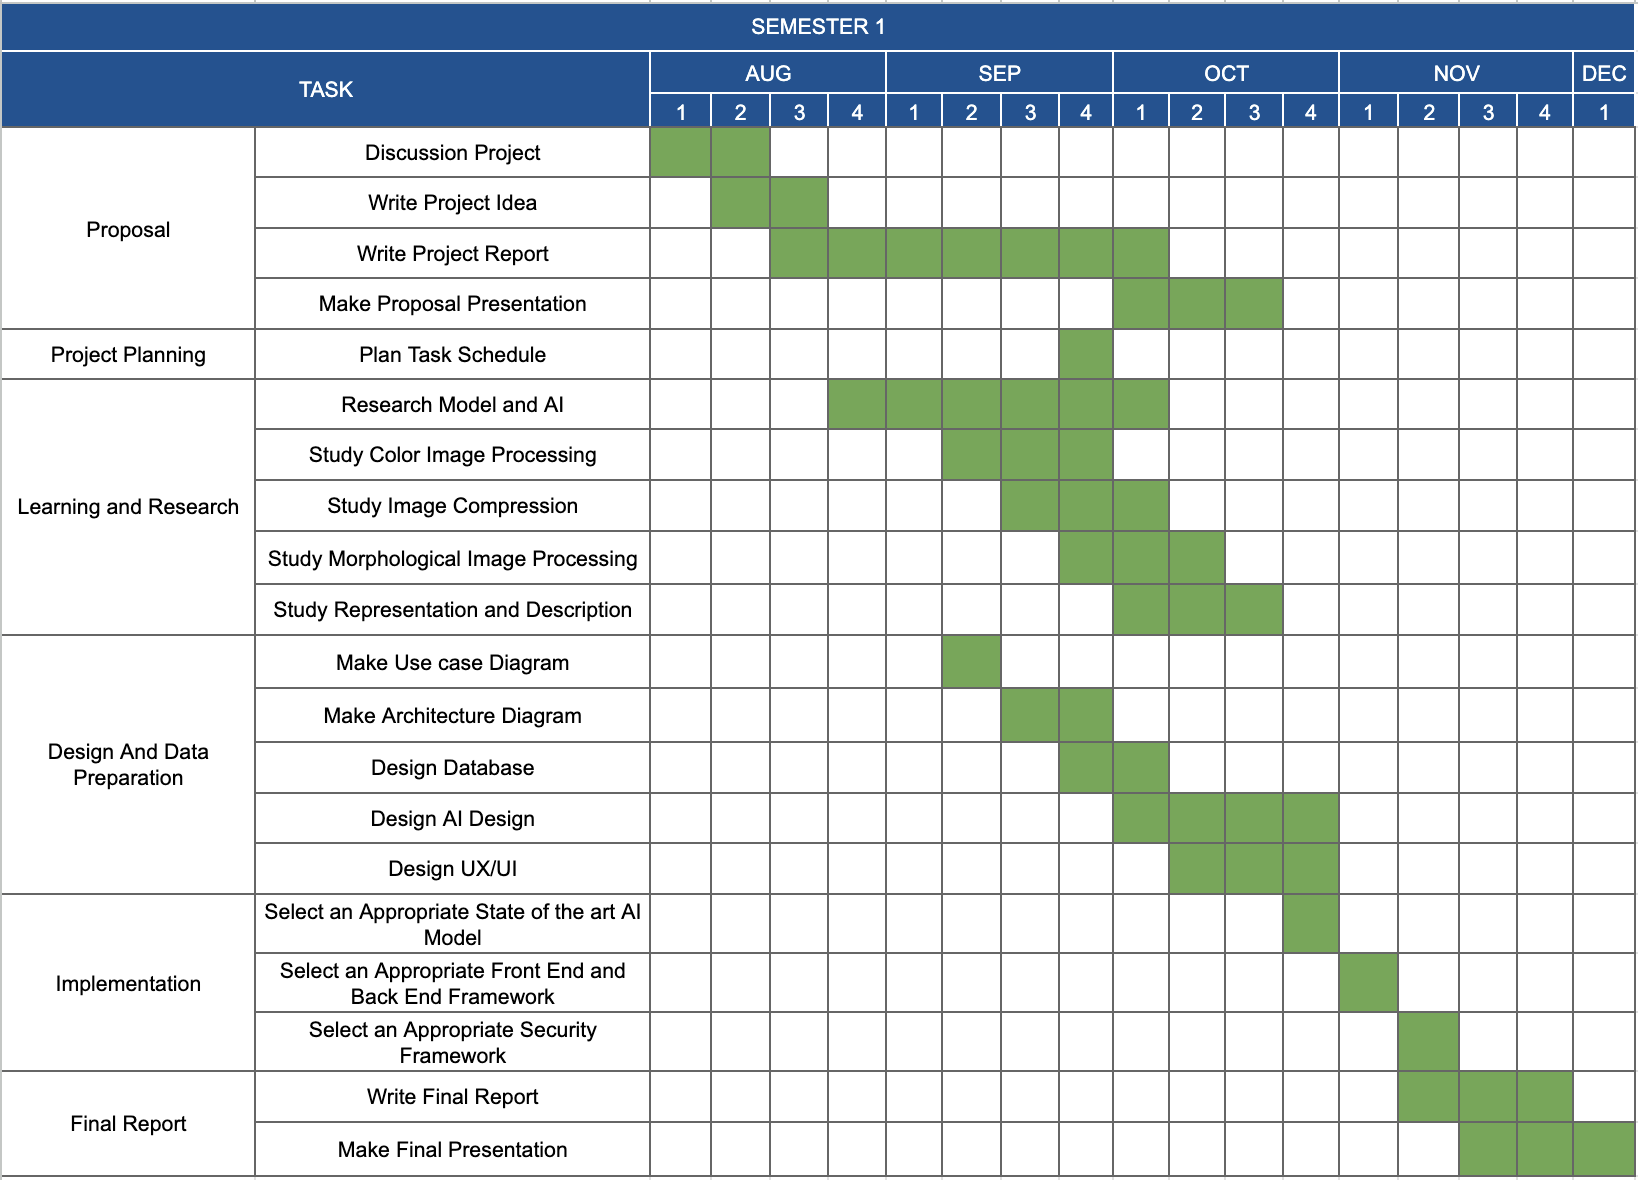
\includegraphics[width=10cm]{./assets/schedule-term1.png}}
\caption{Schedule for first semester}\label{fig:schedule-1}
\end{figure}

For the second semester, our project focus on implementing the form extractor and generative AI for the process of detect a form. We also focus on web application development and integrate a web application with the form extractor. also including the testing phase a system evaluation.

\begin{figure}[!h]
\centering
\fbox{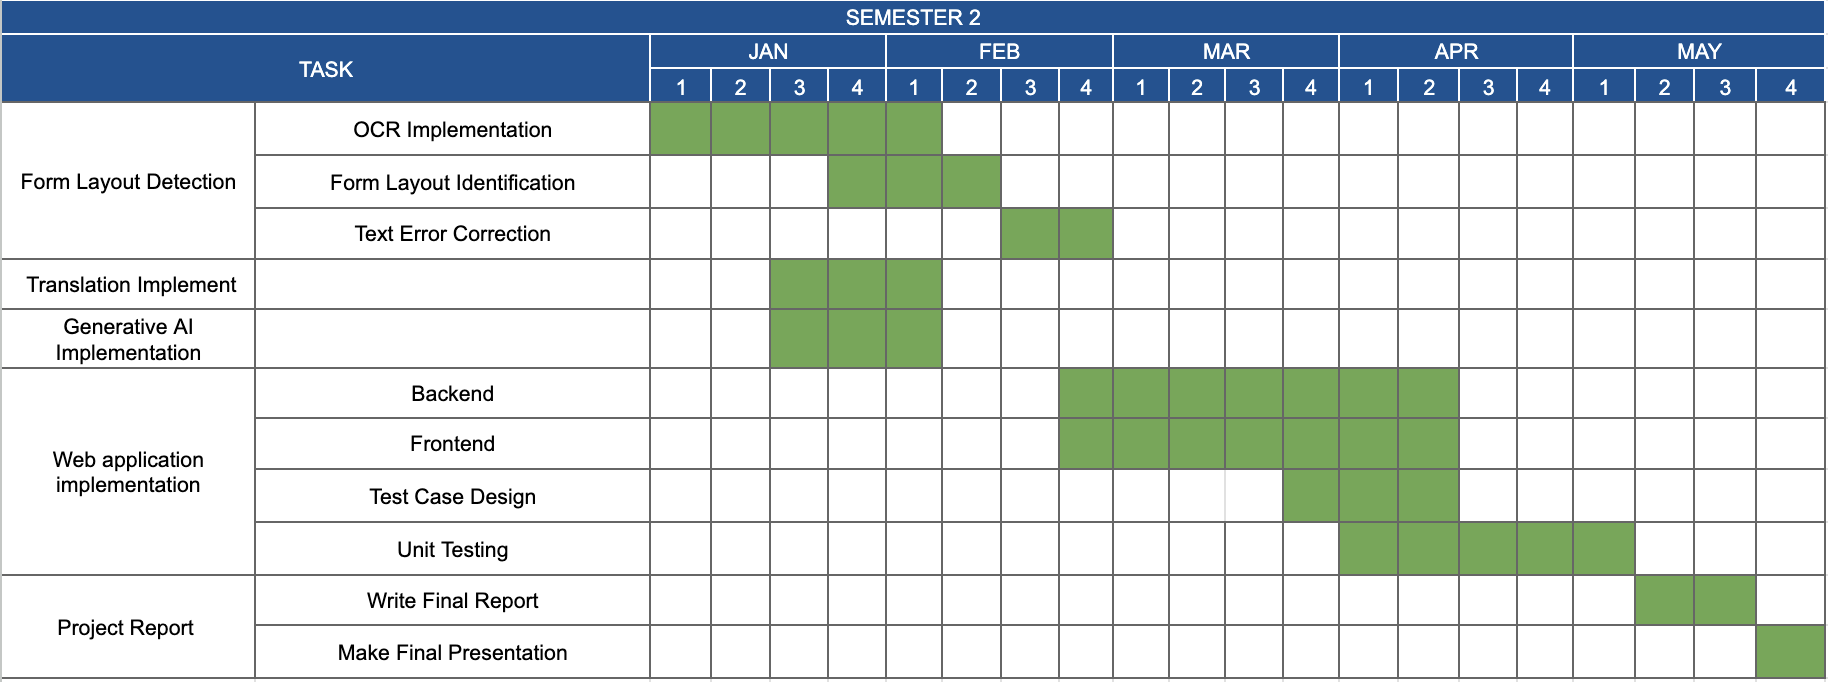
\includegraphics[width=10cm]{./assets/schedule-term2.png}}
\caption{Schedule for second semester}\label{fig:schedule-2}
\end{figure}

\section{Expected Outcomes}
This project aims to develop a fully functional web application that able to converting a paper-based form or pdf form into a web-based form by utilizing a generative AI for generate a data type of form label. And the web application should reduce a time developer have spend when they converting a form.

%%%%%%%%%%%%%%%%%%%%%%%%%%%%%%%%%%%%%%%%%%%%%%%%%%%%%%%%%%%%
%%%%%%%%%%%%%%  Literature Review %%%%%%%%%%%%%%%%%%%%%%%%%%
%%%%%%%%%%%%%%%%%%%%%%%%%%%%%%%%%%%%%%%%%%%%%%%%%%%%%%%%%%%%
\chapter{Background Theory and Related Work}

THIS IS AN EXAMPLE. ALL SECTIONS BELOW ARE OPTIONAL. PLEASE CONSULT YOU ADVISOR AND DESIGN YOUR OWN SECTION

\emph{\textthai{หัวข้อต่าง ๆ ในแต่ละบทเป็นเพียงตัวอย่างเท่านั้น หัวข้อที่จะใส่ในแต่ละบทขึ้นอยู่กับโปรเจคของนักศึกษาและอาจารย์ที่ปรึกษา}}

This is how you add website url. -> \url{http://www.cpe.kmutt.ac.th}

Explain theory, algorithms, protocols, or existing research works and tools related to your work.

You can cite your references like this -> \cite{santi05b}  or multiplie cite like this -> \cite{bworld,hypersense}

\section{Recommender Systems}

\begin{table}[!h]
\caption{test table method1}\label{tbl:method1}
\begin{tabular}{c|c|l|rr} \hline\hline
Center & Center & left aligned & Right & Right aligned \\ \hline\hline
Center & Center & left aligned & Right & Right aligned \\ \hline
Center & Center & left aligned & Right & Right aligned \\ 
Center & Center & left aligned & Right & Right aligned \\ \hline
Center & Center & left aligned & Right & Right aligned \\ \hline\hline
\end{tabular}
\end{table}

Tables should always on the left.
\section{Text Processing Algorithms}
\subsection{Algorithm I}
\subsubsection{test}

% Can define this in the preamble..
You can place the figure and refer to it as Figure~\ref{fig:model2}.
The figure and table numbering will be run and updated automatically when you add/remove tables/figures from the document.

\begin{figure}[!h]\centering
\setlength{\fboxrule}{0.2mm} % can define this in the preamble
\setlength{\fboxsep}{1cm}
\fbox{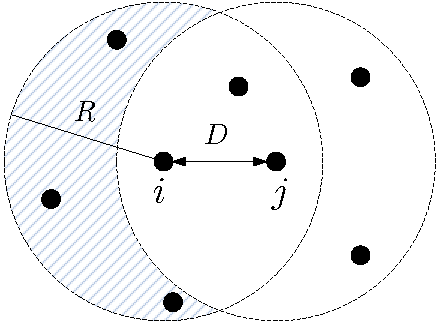
\includegraphics[width=5cm]{./model2.pdf}}
\caption{The network model}\label{fig:model2}
\end{figure}

 
\subsection{Algorithm II}
Add more subsections as you want.
\subsubsection{Step I}
\subsubsection{Step II}
This is the farthest level of subsection we permitted. (We support only 4th level)

\section{Development Tools}

%%%%%%%%%%%%%%%%%%%%%%%%%%%%%%%%%%%%%%%%%%%%%%%%%%%%%
%%%%%%%%%%%%%%CHAPTER 3 DESIGN AND METHODOLOGY%%%%%%%%%%%%%%%%
%%%%%%%%%%%%%%%%%%%%%%%%%%%%%%%%%%%%%%%%%%%%%%%%%%%%%
\chapter{DESIGN AND METHODOLOGY}

This chapter will cover the features, architecture, functionalities, design methods, and
diagrams of our web application. We will delve into the details of the application’s
functionality and architecture.

\section{Project Functionality}

\subsection{System Requirements}

\begin{itemize}
 \item The web application must allow users to log in with email and password. 
 \item The web application must allow the user to upload a form file to the system.
 \item The web application must allow users to fill the form without login.
 \item The web application must allow users to view the data of the form.
 \item The web application must allow users to edit the form before publishing.
 \item The web application must allow users to delete the form.
 \item The web applications must provide the option for all logged-in users to logout.
\end{itemize}

\subsection{Feature List}

\subsubsection{Paper-Based Form Analysis System}

The Paper-Based Form Analysis System will extract all the text from the document that is uploaded by the user via a web application. The system will then analyze the form’s pattern ,extract the input labels, translate the text into English, and send the translated information to a generative AI for data type generation.

\subsubsection{Form Schema generator System}

The Form Schema generator System will receive information from the Paper-Based Form Analysis System and Form Schema generator System must be able to generate a form schema that compatible with a form library.

\subsubsection{Web Form System}

The Digital Form System must enable users to complete the form, store the data in the database, and see the data created by the form owner.

\subsubsection{Registration and Authentication System}

The Registration and Authentication System must enable a user to register and login to the system by using only email and password. This including a forgot password and the  OTP for reset password.	

\section{Use Case Diagram}

From the Figure \ref{fig:use-case} The diagram shows a relationship between the user and the system by using a use case diagram. The user of the system is a developer that needs to transform a paper-base form into web application form and the user who going to fill the form. The system consists of 3 different systems, which are paper-based form analysis systems, form schema generator systems, web form systems and registration and authentication systems. The user can upload a paper-based form to the system, and the system will transform the form into a web-based form.

\begin{figure}[!h]
\centering
\fbox{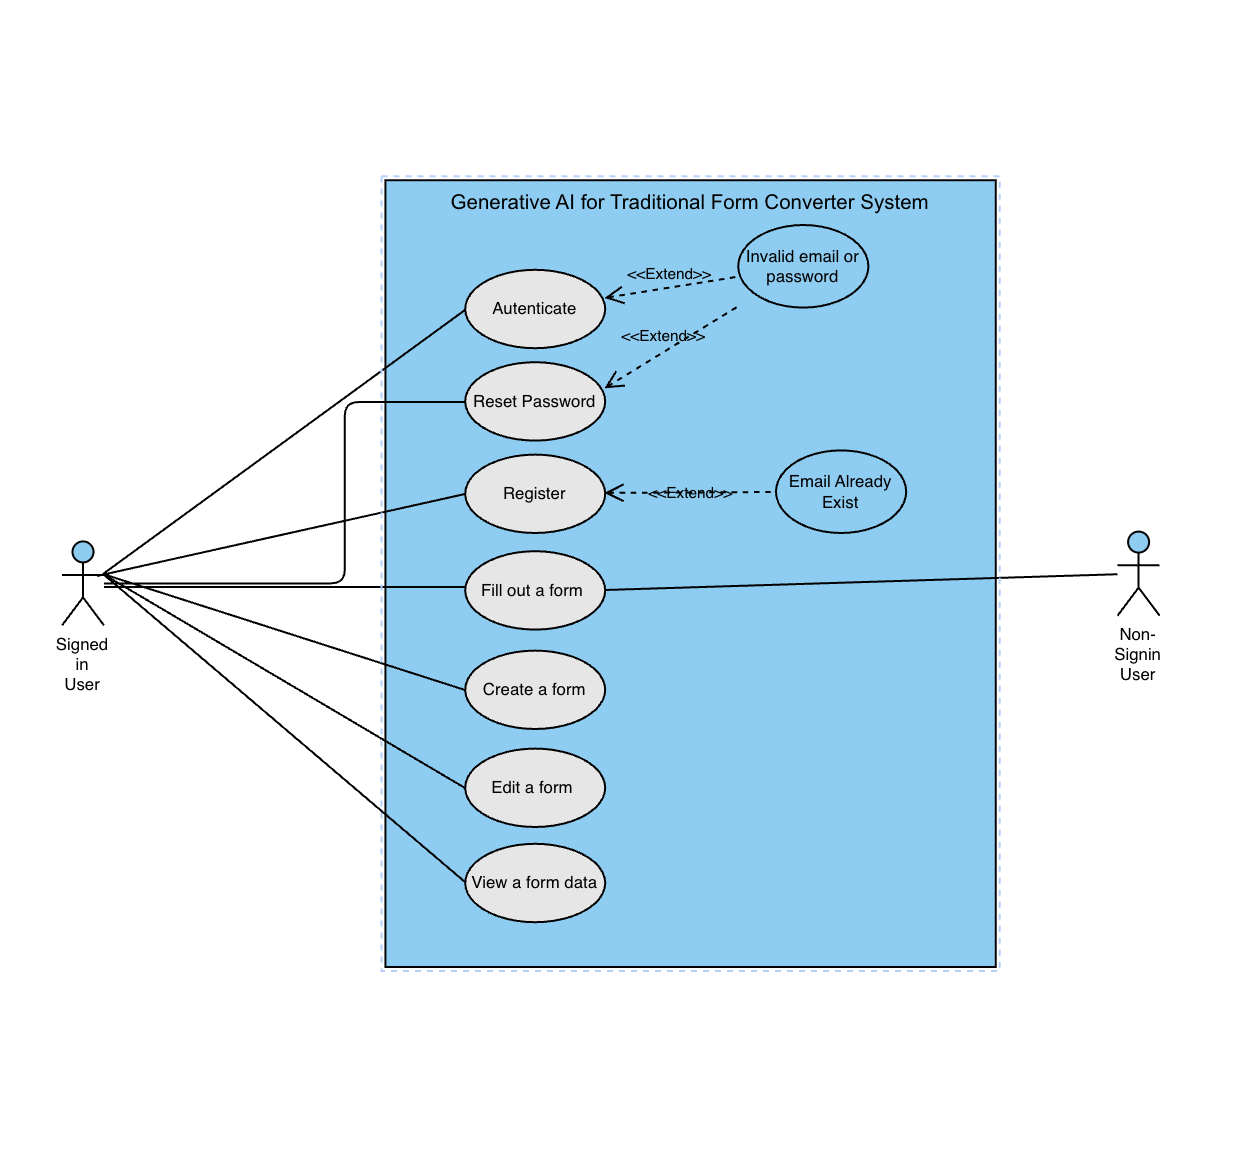
\includegraphics[width=10cm]{./assets/usecase.png}}
\caption{Use case diagram}\label{fig:use-case}
\end{figure}

\section{Use Case Narrative}

\subsection{Autentication}

\textbf{Use Case Name:} Autentication \\
\textbf{Actors:} Form Creator and Required Login User \\
\textbf{Goal:} Users log in to the system. \\
\textbf{Preconditions:} User is registered

Main Success Scenario: 

\begin{enumerate}
    \item User access the website.
    \item User enter a email and password.
    \item User submit a email and password.
    \item System authenticate and navigate to the home page.
\end{enumerate}

\subsection{Register}

\textbf{Use Case Name:} Register \\
\textbf{Actors:} Form Creator and Required Login User \\
\textbf{Goal:} Users register to a system. \\
\textbf{Preconditions:} User does not have an account

Main Success Scenario: 

\begin{enumerate}
    \item User access the website.
    \item User click to create a new account.
    \item User enter an email and password and personal information.
    \item User submit information.
    \item System saves user information and navigates users to the login page.

\end{enumerate}

\subsection{Create a form}

\textbf{Use Case Name:} Create a form \\
\textbf{Actors:} Form Creator\\
\textbf{Goal:} Create a form by upload the form file. \\
\textbf{Preconditions:} User has logged in.

Main Success Scenario: 

\begin{enumerate}
    \item User go to home page.
    \item User click at upload a form.
    \item User select a file to upload.
    \item System will process the file and navigate users to the edit form page to confirm a form before publishing.
   
\end{enumerate}

\subsection{Edit a form}

\textbf{Use Case Name:} Edit a form \\
\textbf{Actors:} Form Creator\\
\textbf{Goal:} Edit a form to make a change.\\
\textbf{Preconditions:} User has logged in.

Main Success Scenario: 

\begin{enumerate}
    \item User go to home page.
    \item User click at edit a form at the form user need to make change.
    \item User make change a form.
    \item User click back to the previous page.
    \item System will process autosave and navigate users to the previous page.
\end{enumerate}


\subsection{View a form data}

\textbf{Use Case Name:} View a form data \\
\textbf{Actors:} Form Creator\\
\textbf{Goal:}View the data that user have input\\
\textbf{Preconditions:} User has logged in.

Main Success Scenario: 

\begin{enumerate}
    \item User go to home page.
    \item User click at view a data of the form.
    \item User can see a form data
\end{enumerate}

\subsection{Fill up the form}

\textbf{Use Case Name:} Fill up the form \\
\textbf{Actors:} Required Login Users and Anonymous User \\
\textbf{Goal:} Add a new data to the form \\
\textbf{Preconditions:} User has logged in or non-login user.

Main Success Scenario: 

\begin{enumerate}
    \item User access a form via the public link
    \item User fill up a form.
    \item User submit a form data.
    \item System will save the data and navigate to the form page again.
\end{enumerate}

Alternate scenario (user access the form required a login without login):

\begin{enumerate}
    \item User access a form via the public link
    \item System will navigate to the login page After login completes the user will redirect back to the form page.
\end{enumerate}


\section{Activity Diagram}

From Figure \ref{fig:activity-diagram}  The Activity diagram shows the sequence how Generative AI for
Traditional Form Converter System is working.

\begin{figure}[!h]
\centering
\fbox{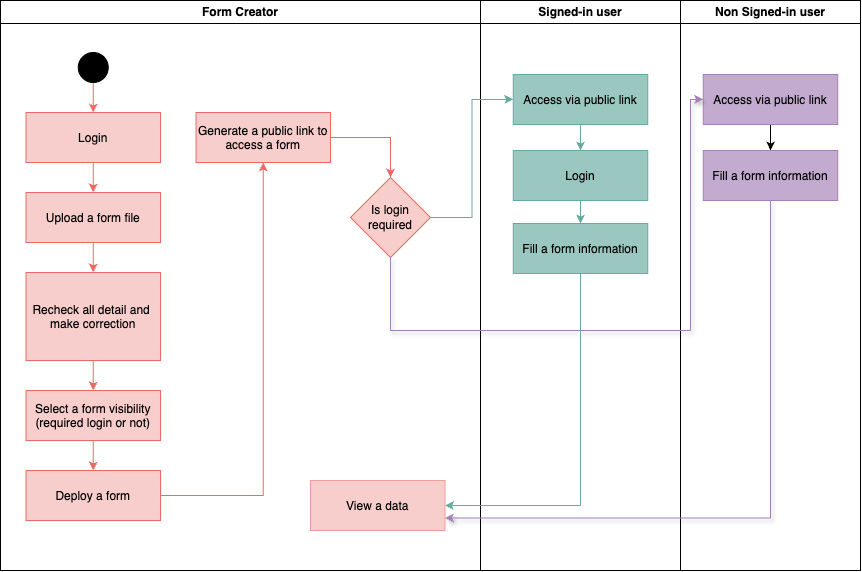
\includegraphics[width=10cm]{./assets/activity-diagram.png}}
\caption{Activity Diagram}\label{fig:activity-diagram}
\end{figure}



\subsection{Form creator}

\begin{itemize}
\item  \textbf{Login:} Form Creator must login before use the system
\item  \textbf{Upload a form file:} After logging in, Form creator must upload a form file to add new form to the system.
\item  \textbf{Recheck all detail and make correction:} In this step, Form creator must check all the information that system has generated and make a correction if incase of error text found.
\item  \textbf{Select a from visibility:} Select a form visibility, whether the form creator need to form to be access by the user who signed-in or anyone can access.
\item  \textbf{Deploy a form and Generate a link:} In this step, the form will be saved and generated a link to allow user to access.

\end{itemize}


\subsection{Signed-in user}

\begin{itemize}
\item  \textbf{Login:} If the form requires login, the user must log into the system.
\item  \textbf{Fill out information:} Once logged in, the user going to fills out the form and submit.
\end{itemize}


\subsection{Non Signed-in user}

\begin{itemize}
\item  \textbf{Fill out information:} If login is not required, the user can directly fill out the form without logging in.
\end{itemize}


\section{System Architecture}

\begin{figure}[!h]
\centering
\fbox{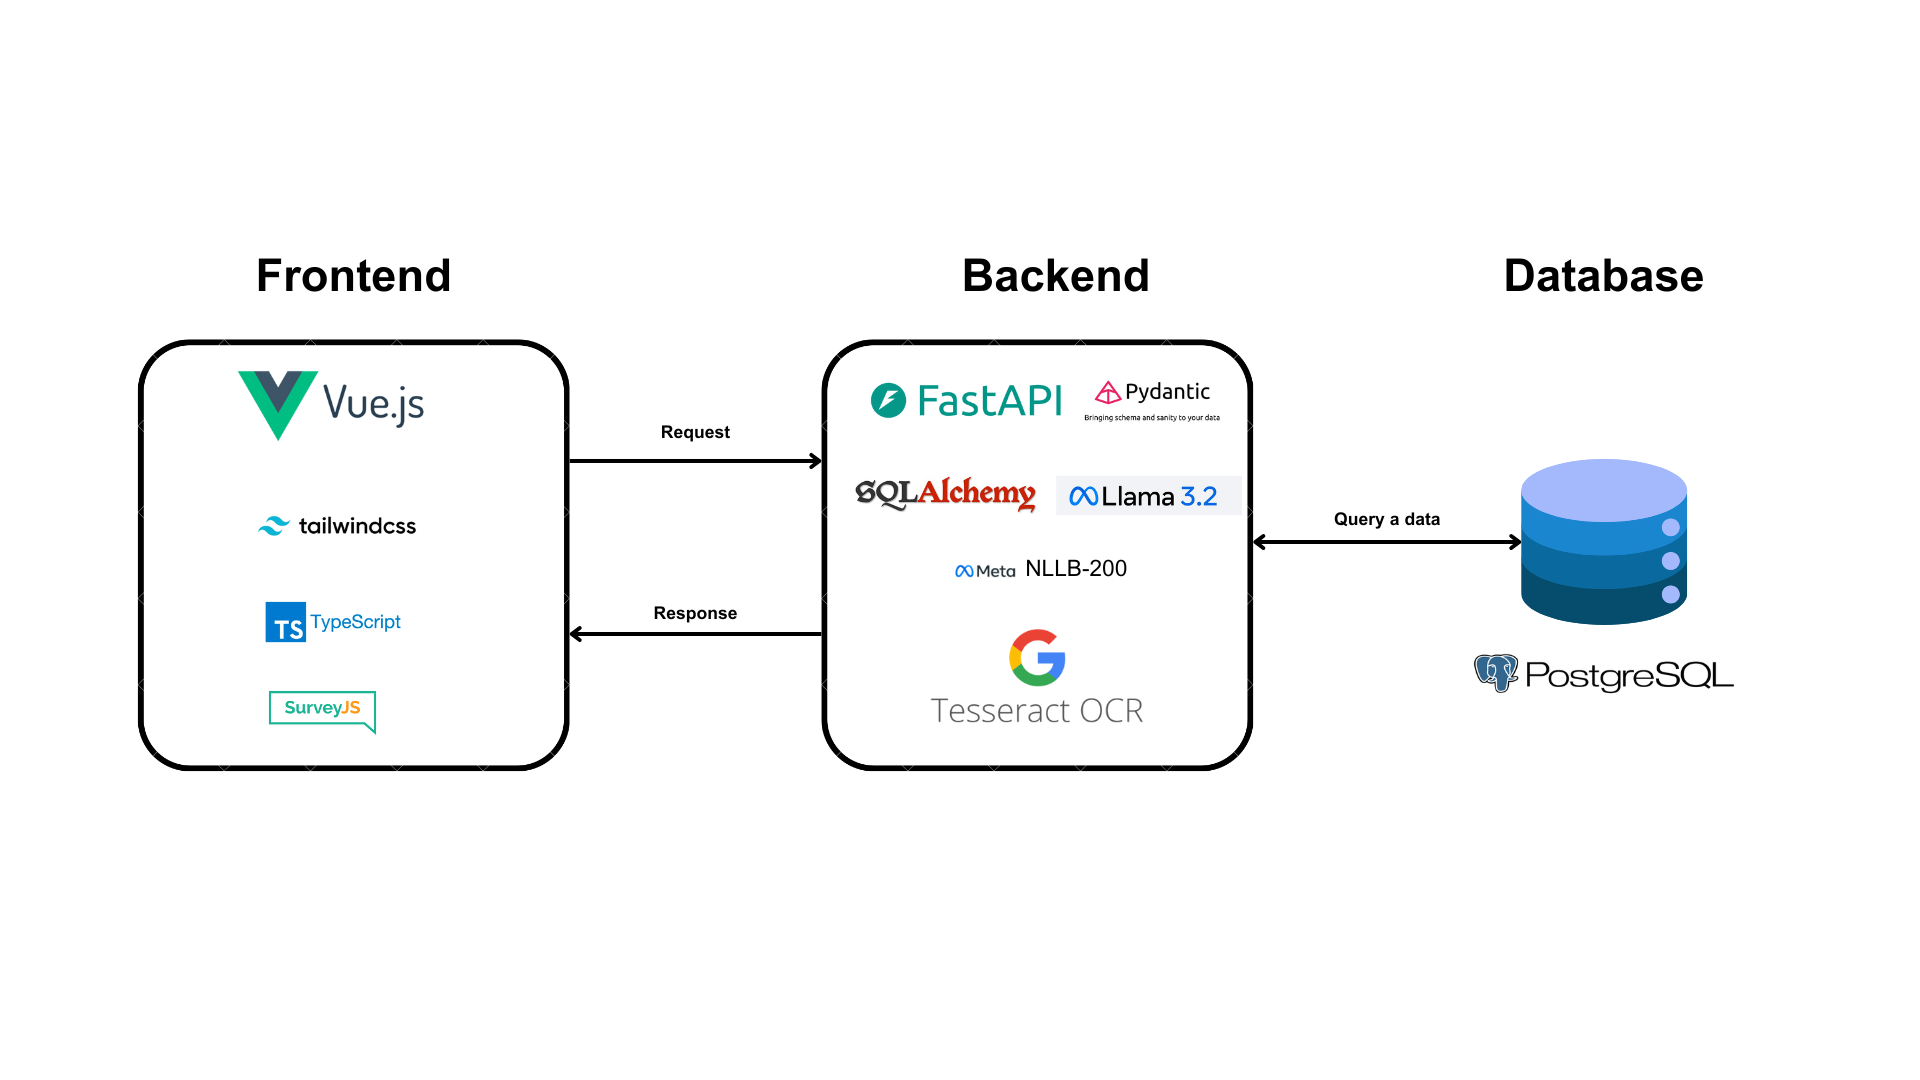
\includegraphics[width=10cm]{./assets/system-arch.png}}
\caption{System Architecture}\label{fig:system-arch}
\end{figure}

Figure \ref{fig:system-arch}, The diagram shown a system architecture in figure above, The System have divided into 3 part which front-end, back-end and database, each part have shown a technology stack, and here are the description of each component

\begin{itemize}
\item  \textbf{VueJS} is a Front-end JavaScript library for building UI
\item \textbf{TailwindCSS} is a CSS framework for styling the UI and used with React
\item \textbf{FastAPI} is a Back-end framework for building REST API
\item \textbf{PostgreSQL}  is a relational database
\item \textbf{Pydantic}  is a python library used for data validation 
\item \textbf{SQLAlchemy} is a Python base Object Relational Mapper (ORM) and SQL Tool kit
\item \textbf{SurveyJS} is a form engine Llibrary
\item \textbf{Meta NLLB-200} is a Model for text translation
\item \textbf{Tesseract OCR} is a OCR for extract text from image
\item \textbf{Llama 3.2} is a generative AI from Facebook
\end{itemize}


\section{Database Design}

Figure \ref{fig:er-diagram} shown a project database design, the system consist three tables in our project database design are user, form, and formresult. table is used to store user data, formresult is used to store a result that the user has filled out, and form table is used to store a form schema.

\begin{figure}[!h]
\centering
\fbox{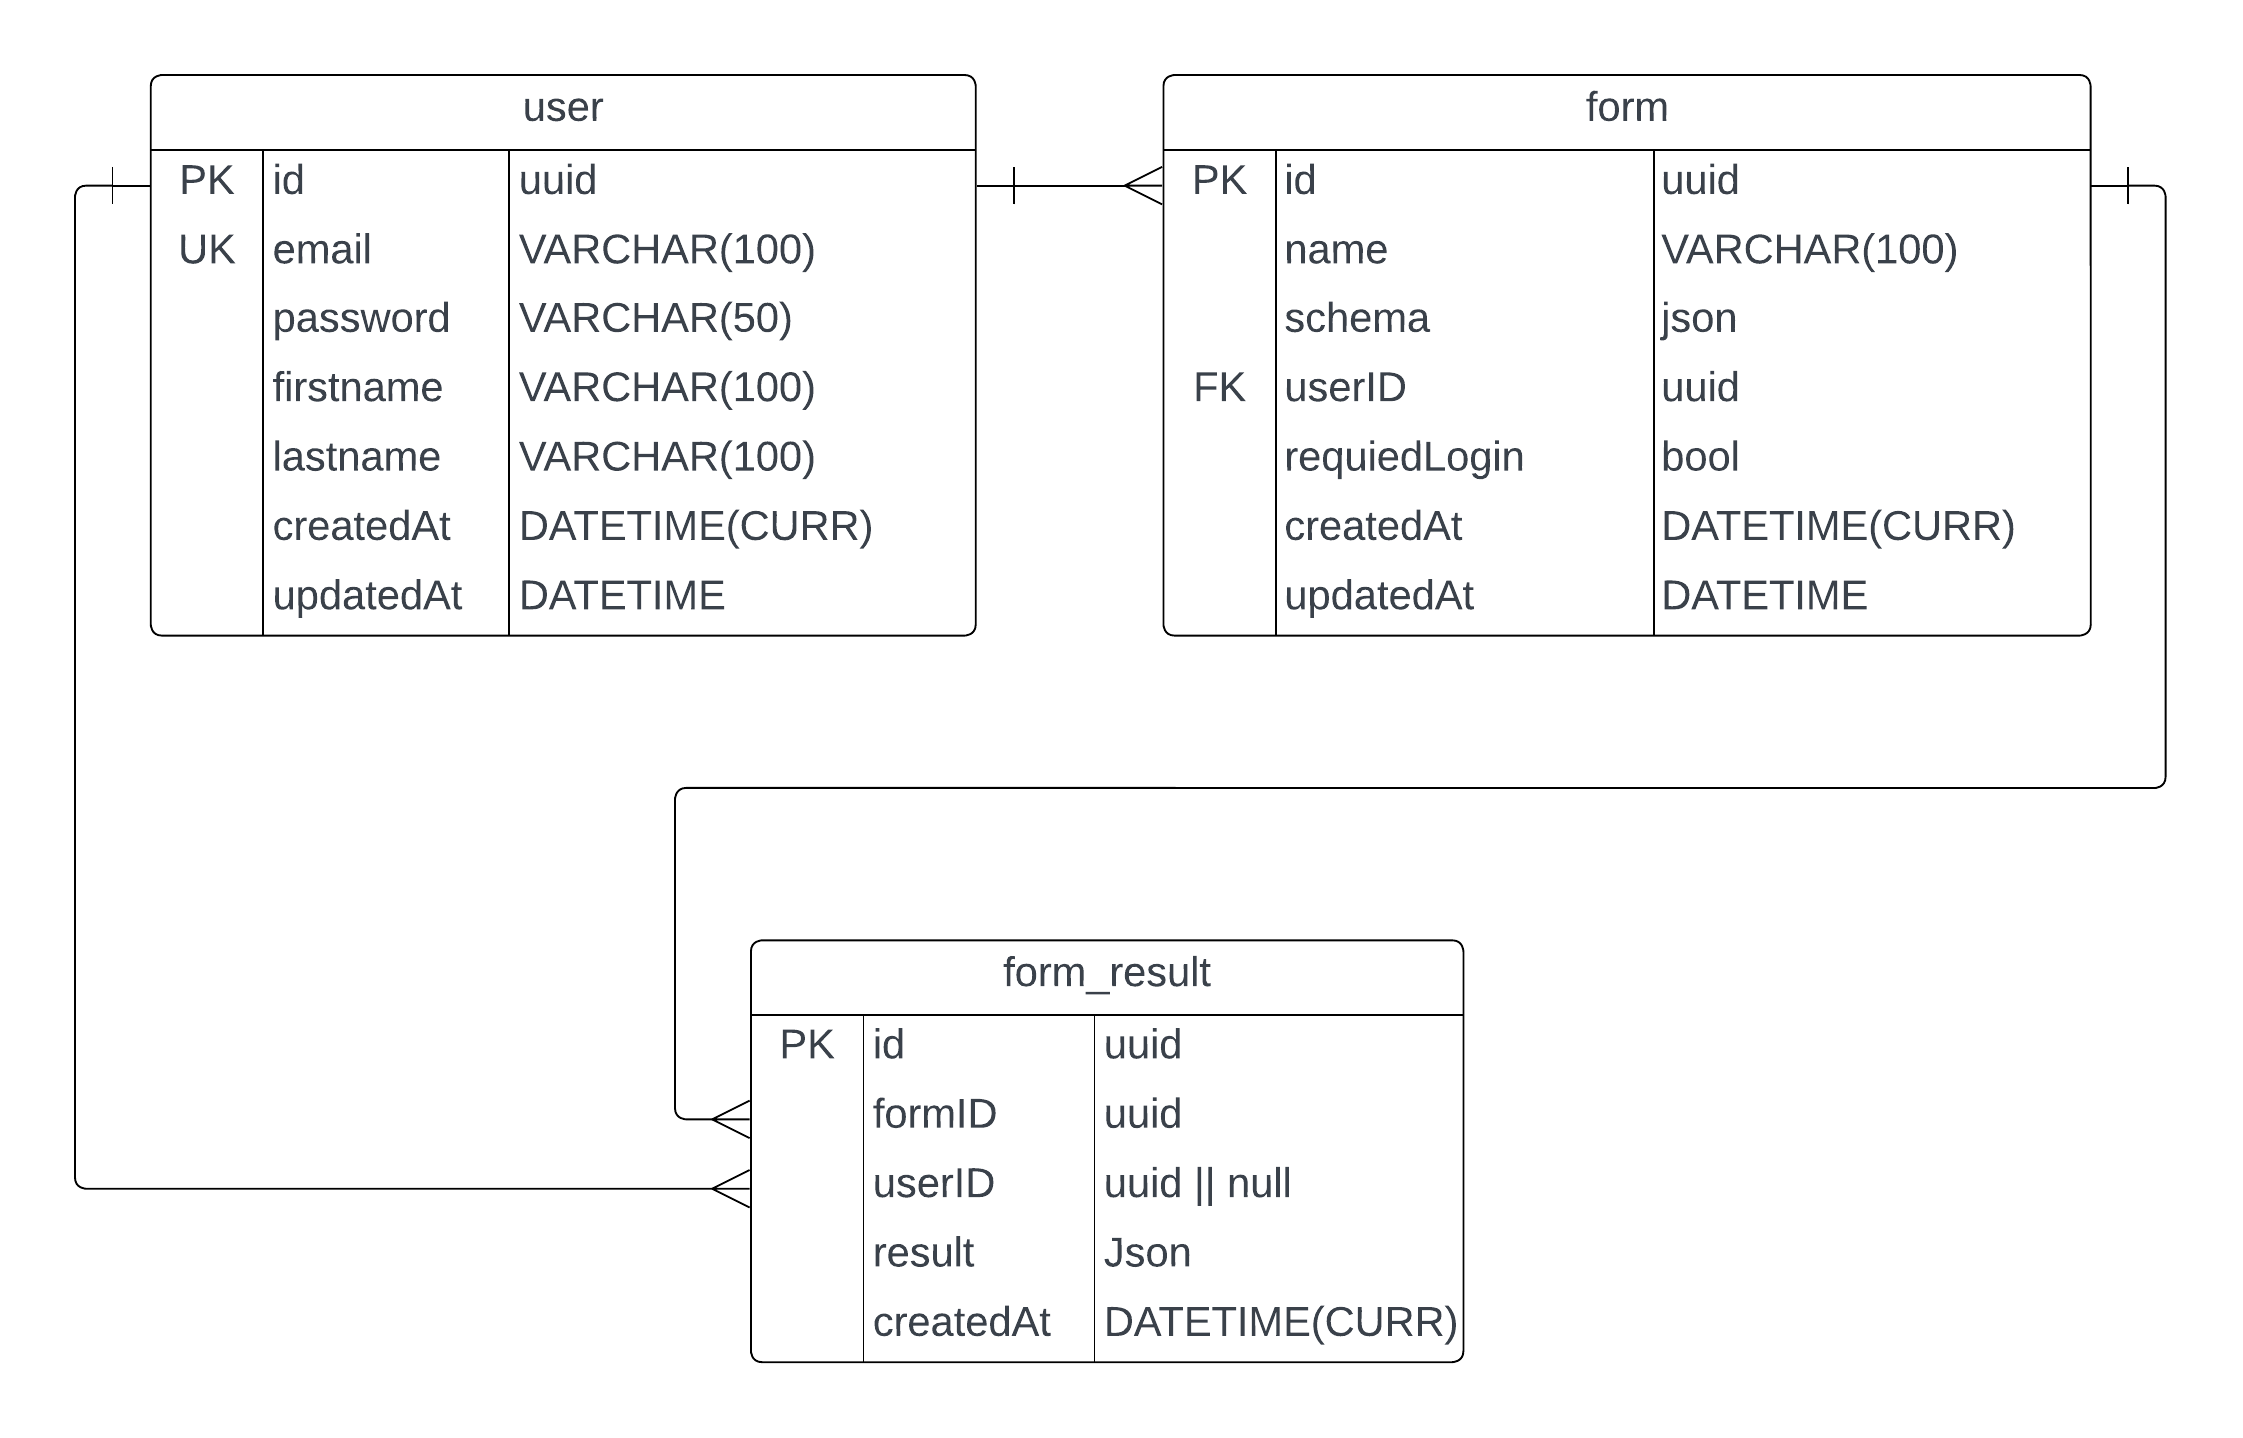
\includegraphics[width=10cm]{./assets/ER-diagram.png}}
\caption{ER Diagram}\label{fig:er-diagram}
\end{figure}

\section{User Interface Design}

\subsection{Login Page}

\begin{figure}[!h]
\centering
\fbox{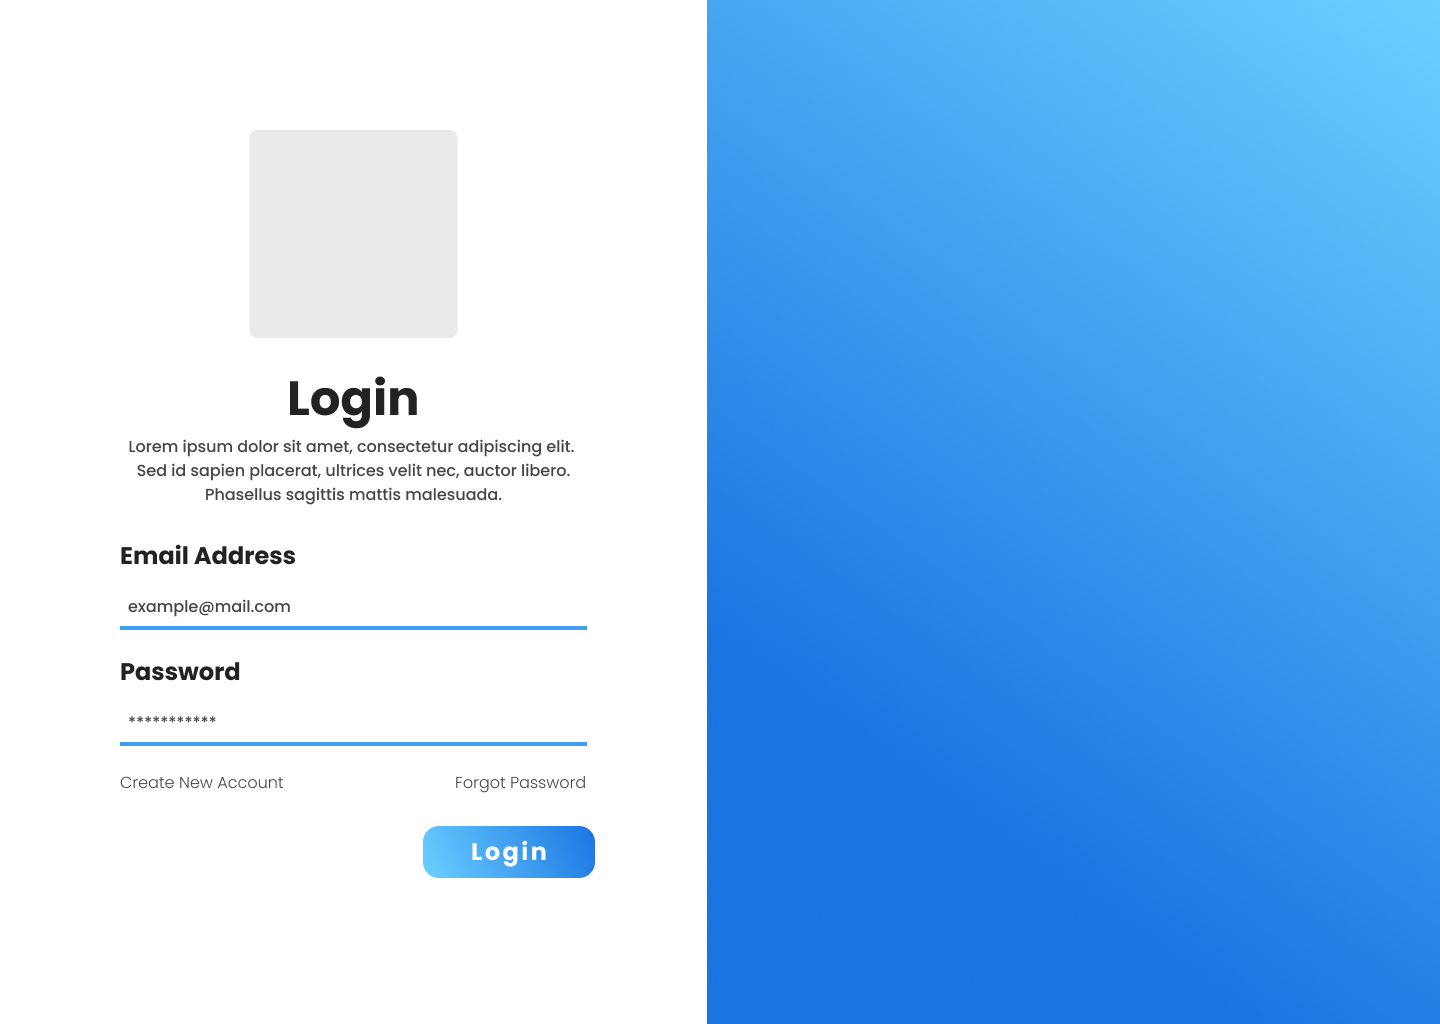
\includegraphics[width= 10cm]{./assets/UI/Login.png}}
\caption{Login Page}\label{fig:login}
\end{figure}

Figure 3.5 represents the login screen of the web application. This page have a email field,  password field and a login button to sent a credential to the back-end system. 

\subsection{Create Your Account }

\begin{figure}[!h]
\centering
\fbox{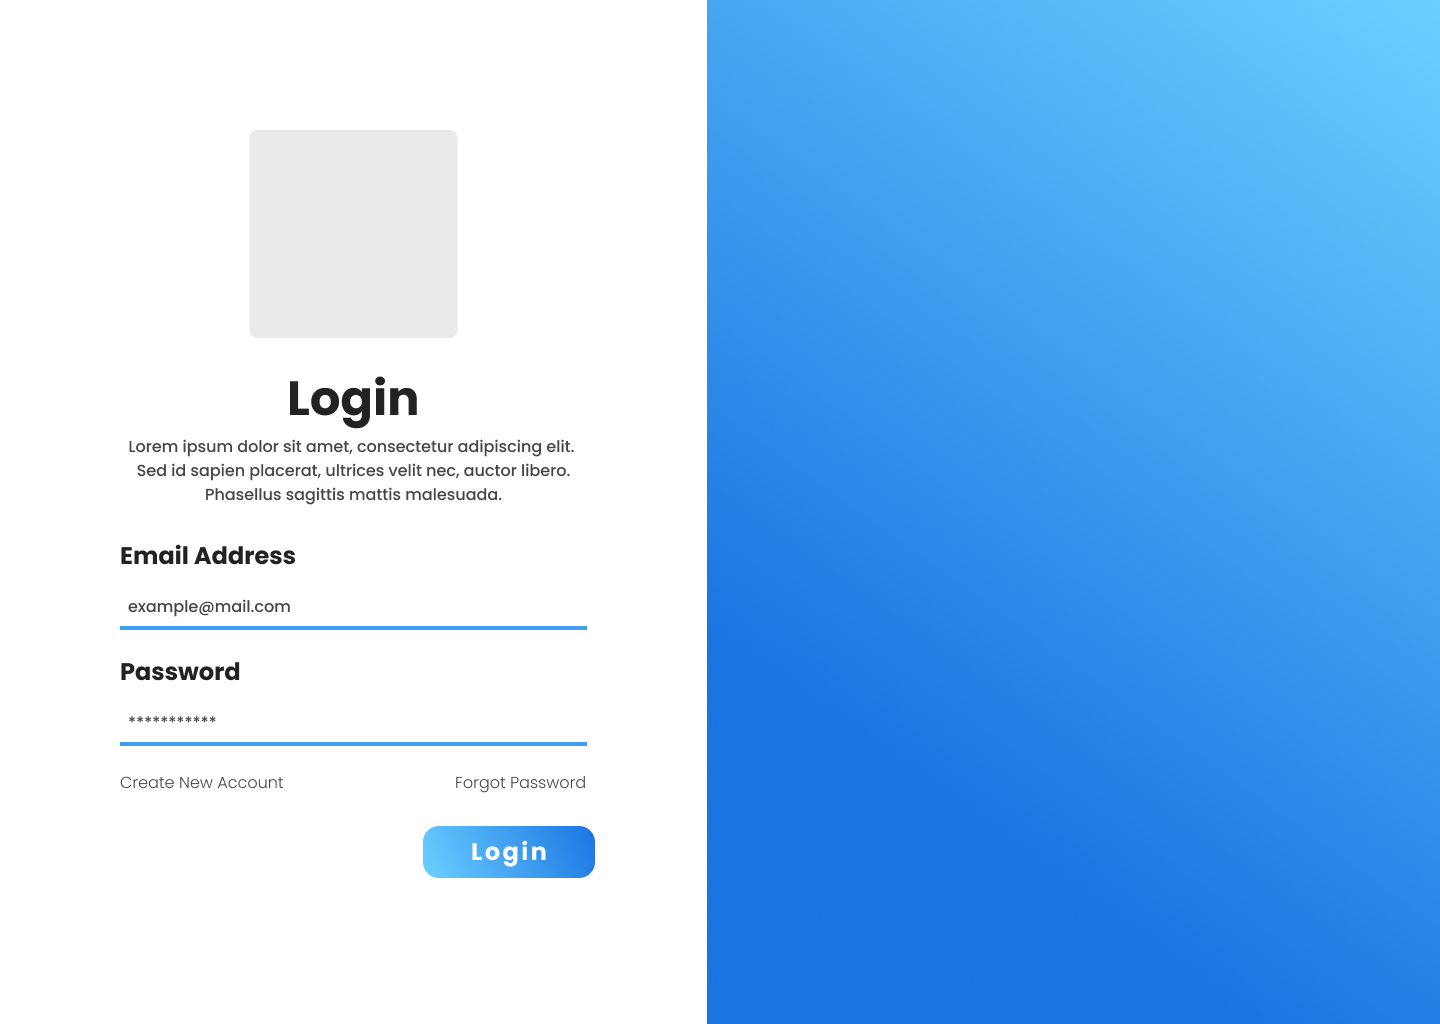
\includegraphics[width= 10cm]{./assets/UI/Login.png}}
\caption{Create Account Page}\label{fig:create-acc}
\end{figure}

Figure 3.6 represents the create account page of the web application. This page allow user to create their own account by the user must provide a following field which is name, email and password.

\subsection{Forgot Password}

At Figure \ref{fig:Forgot-Password} represents the create account page of the web application. When the user forgot their password, The user must navigate to this page by click at forget password from login page. And fill the email address to allow the system sent the One-time password (OTP) to email address. 


\begin{figure}[!h]
\centering
\fbox{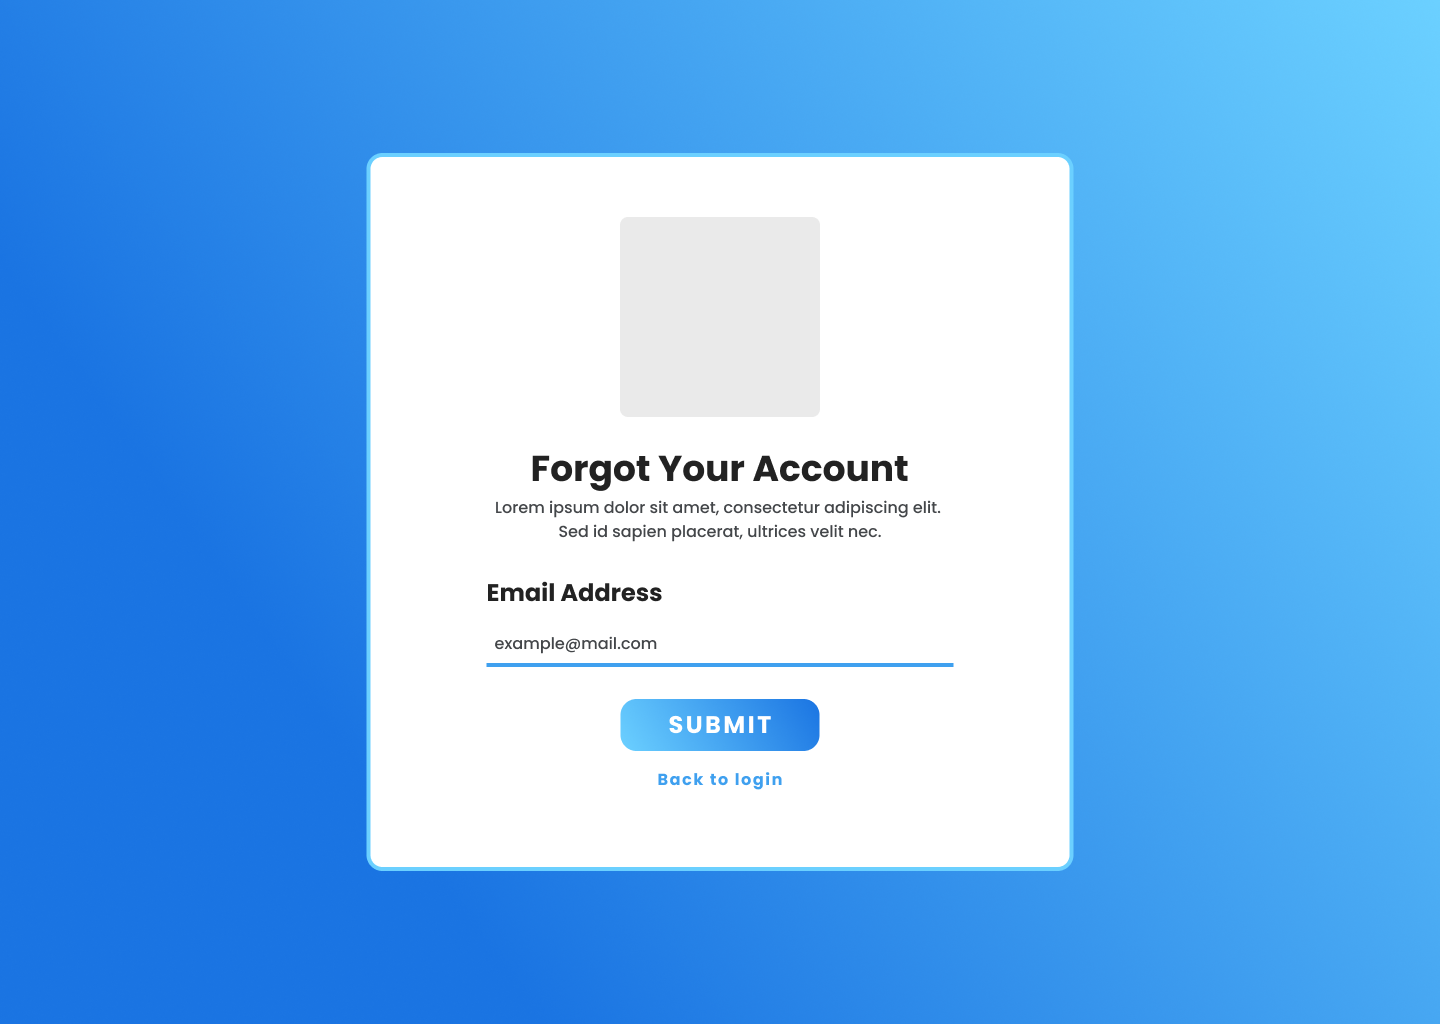
\includegraphics[width= 10cm]{./assets/UI/forgot-password.png}}
\caption{Forgot Password Page}\label{fig:Forgot-Password}
\end{figure}



\begin{figure}[!h]
\centering
\fbox{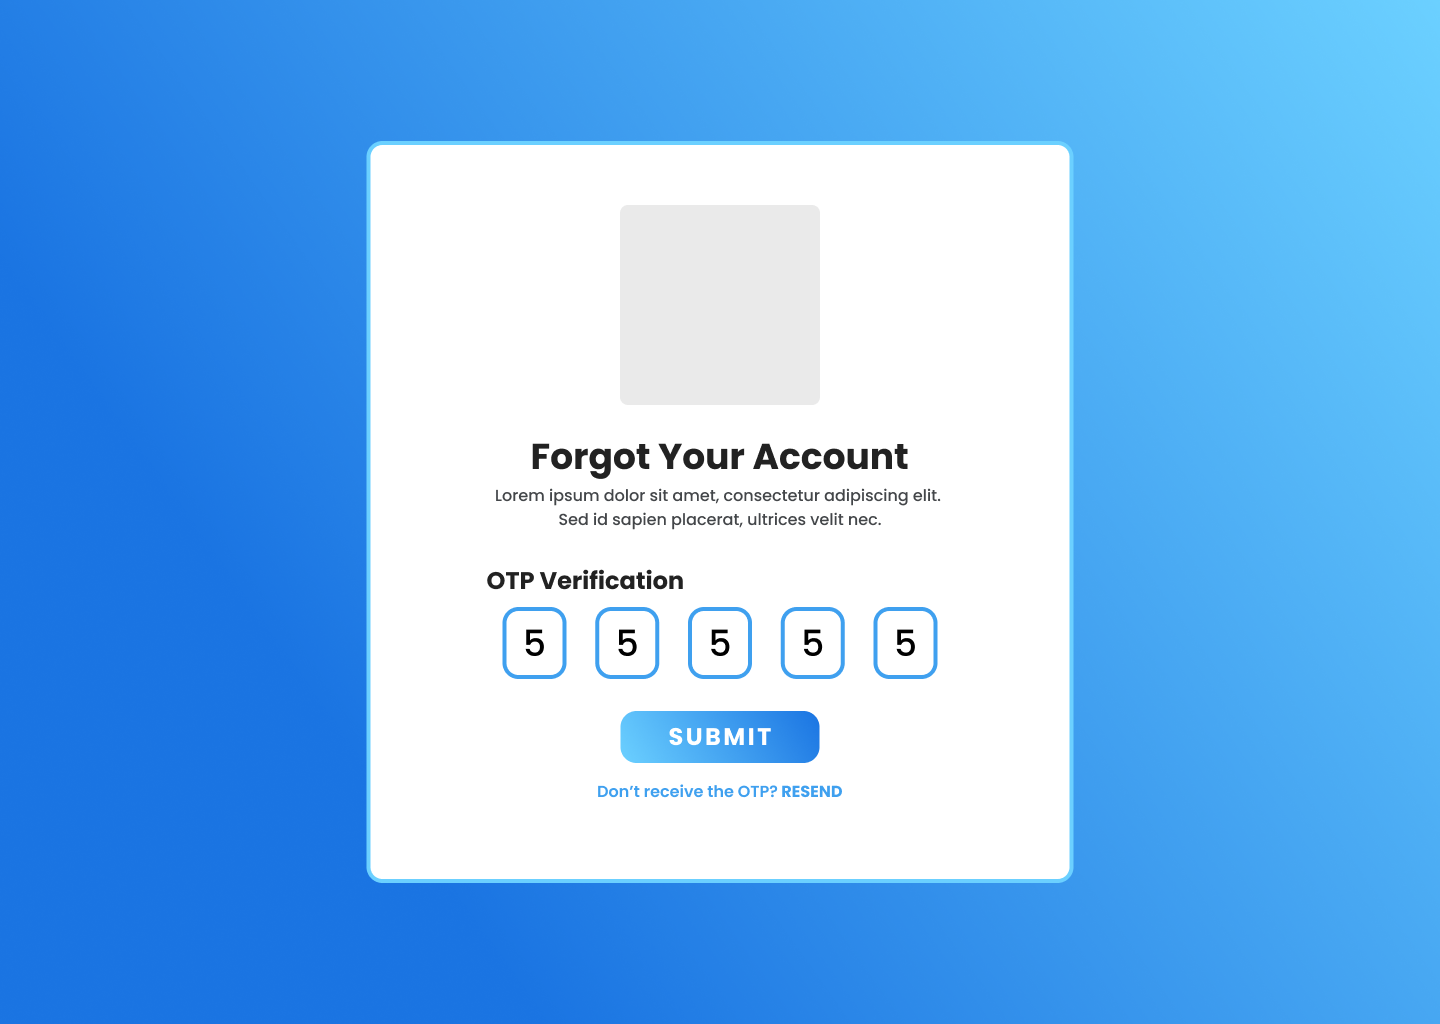
\includegraphics[width= 10cm]{./assets/UI/Forgot-Password-Code.png}}
\caption{Forgot Password Page}\label{fig:Forgot-Password-code}
\end{figure}

\begin{figure}[!h]
\centering
\fbox{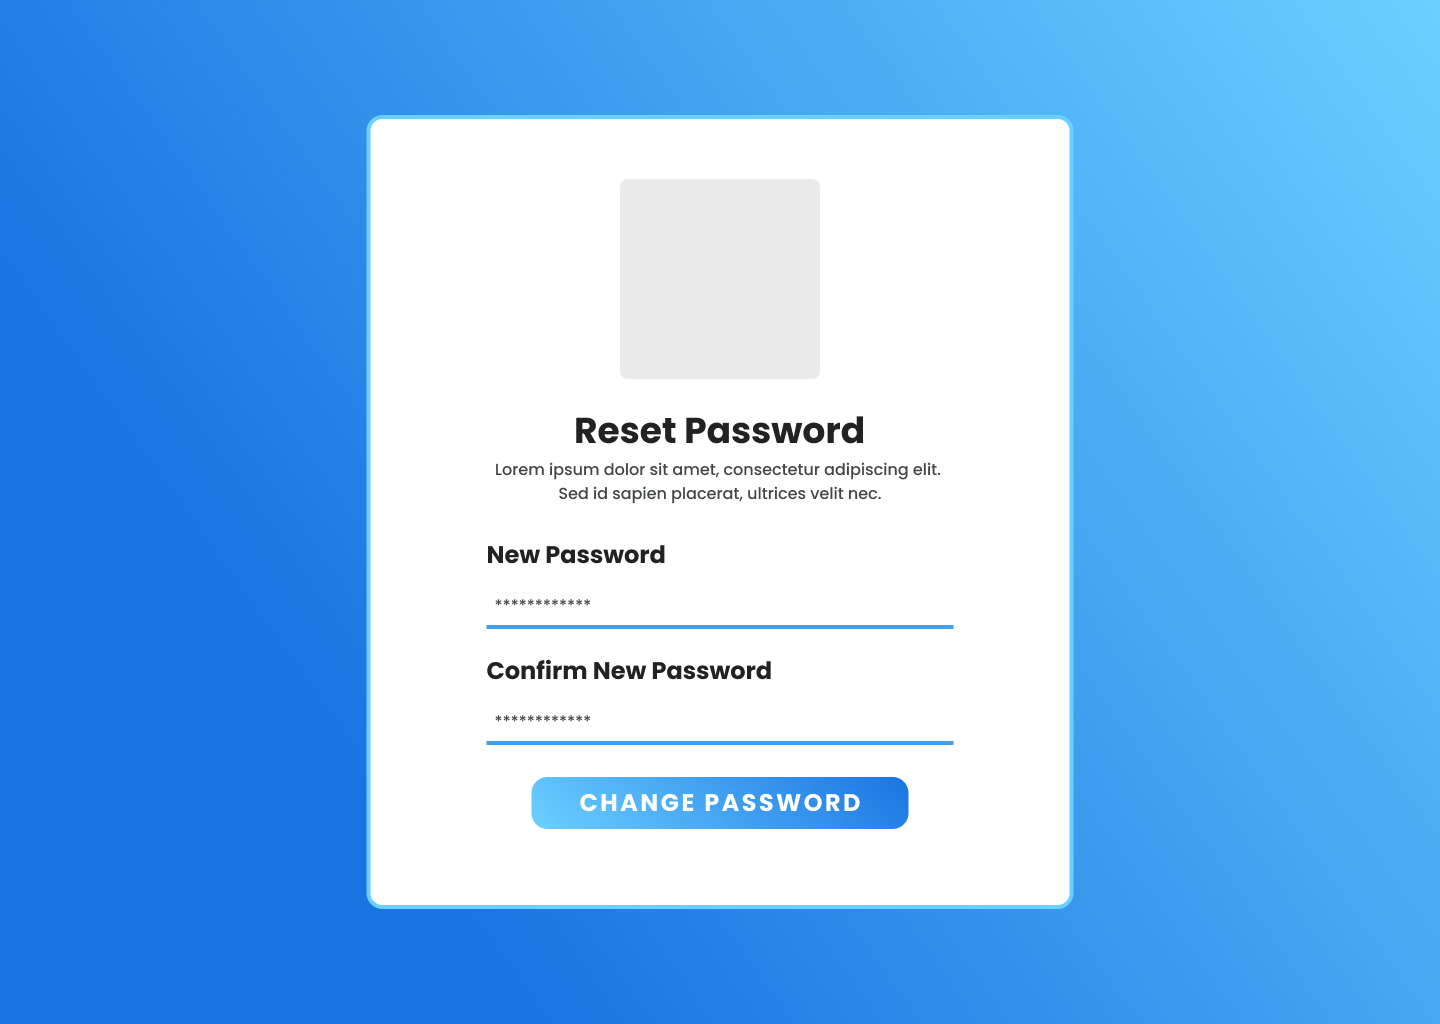
\includegraphics[width= 10cm]{./assets/UI/Reset-password.png}}
\caption{Reset Password Page}\label{fig:Reset Password}
\end{figure}



At the Figure \ref{fig:Forgot-Password-code}, It represents a OTP confirmation page which required a OTP Code that the system have send to the email address. Figure \ref{fig:Reset Password}, It represents a reset password pageIf it success the system will navigate to reset password page for enter a new password.

\newpage
\subsection{Dashboard}

\begin{figure}[!h]
\centering
\fbox{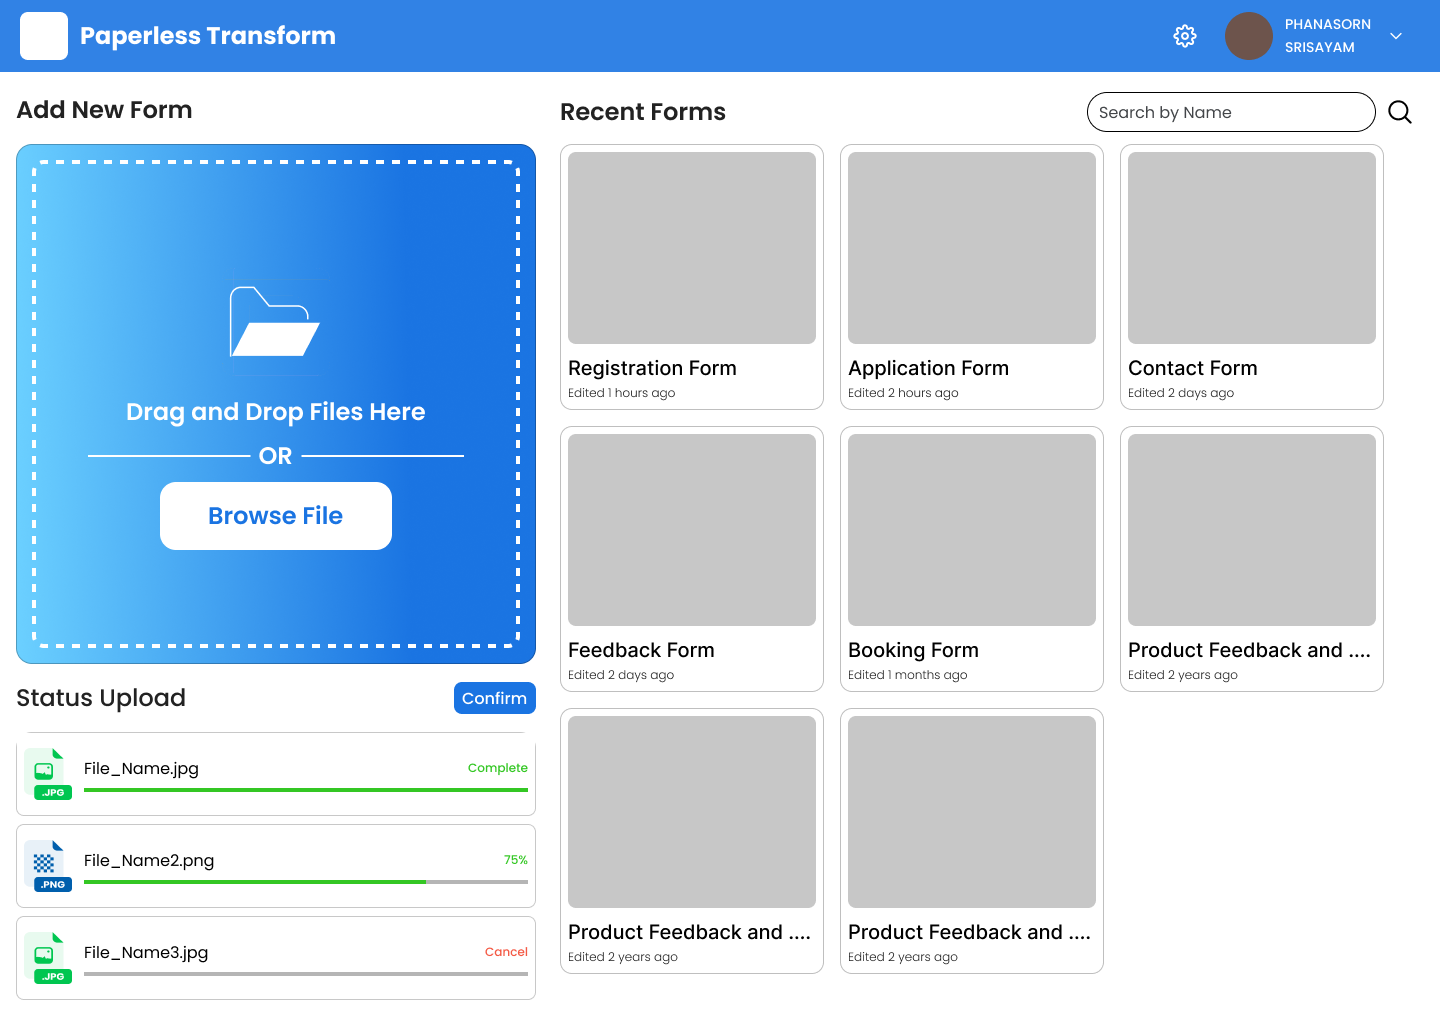
\includegraphics[width= 10cm]{./assets/UI/DashBoard.png}}
\caption{Dashboard Page}\label{fig:Dashboard}
\end{figure}

Figure  \ref{fig:Dashboard}, represents the dashboard page, it will show all the form that user have and the add form section at the left hand side, also have an upload status while file is uploading.

\subsection{Edit Form}

\begin{figure}[!h]
\centering
\fbox{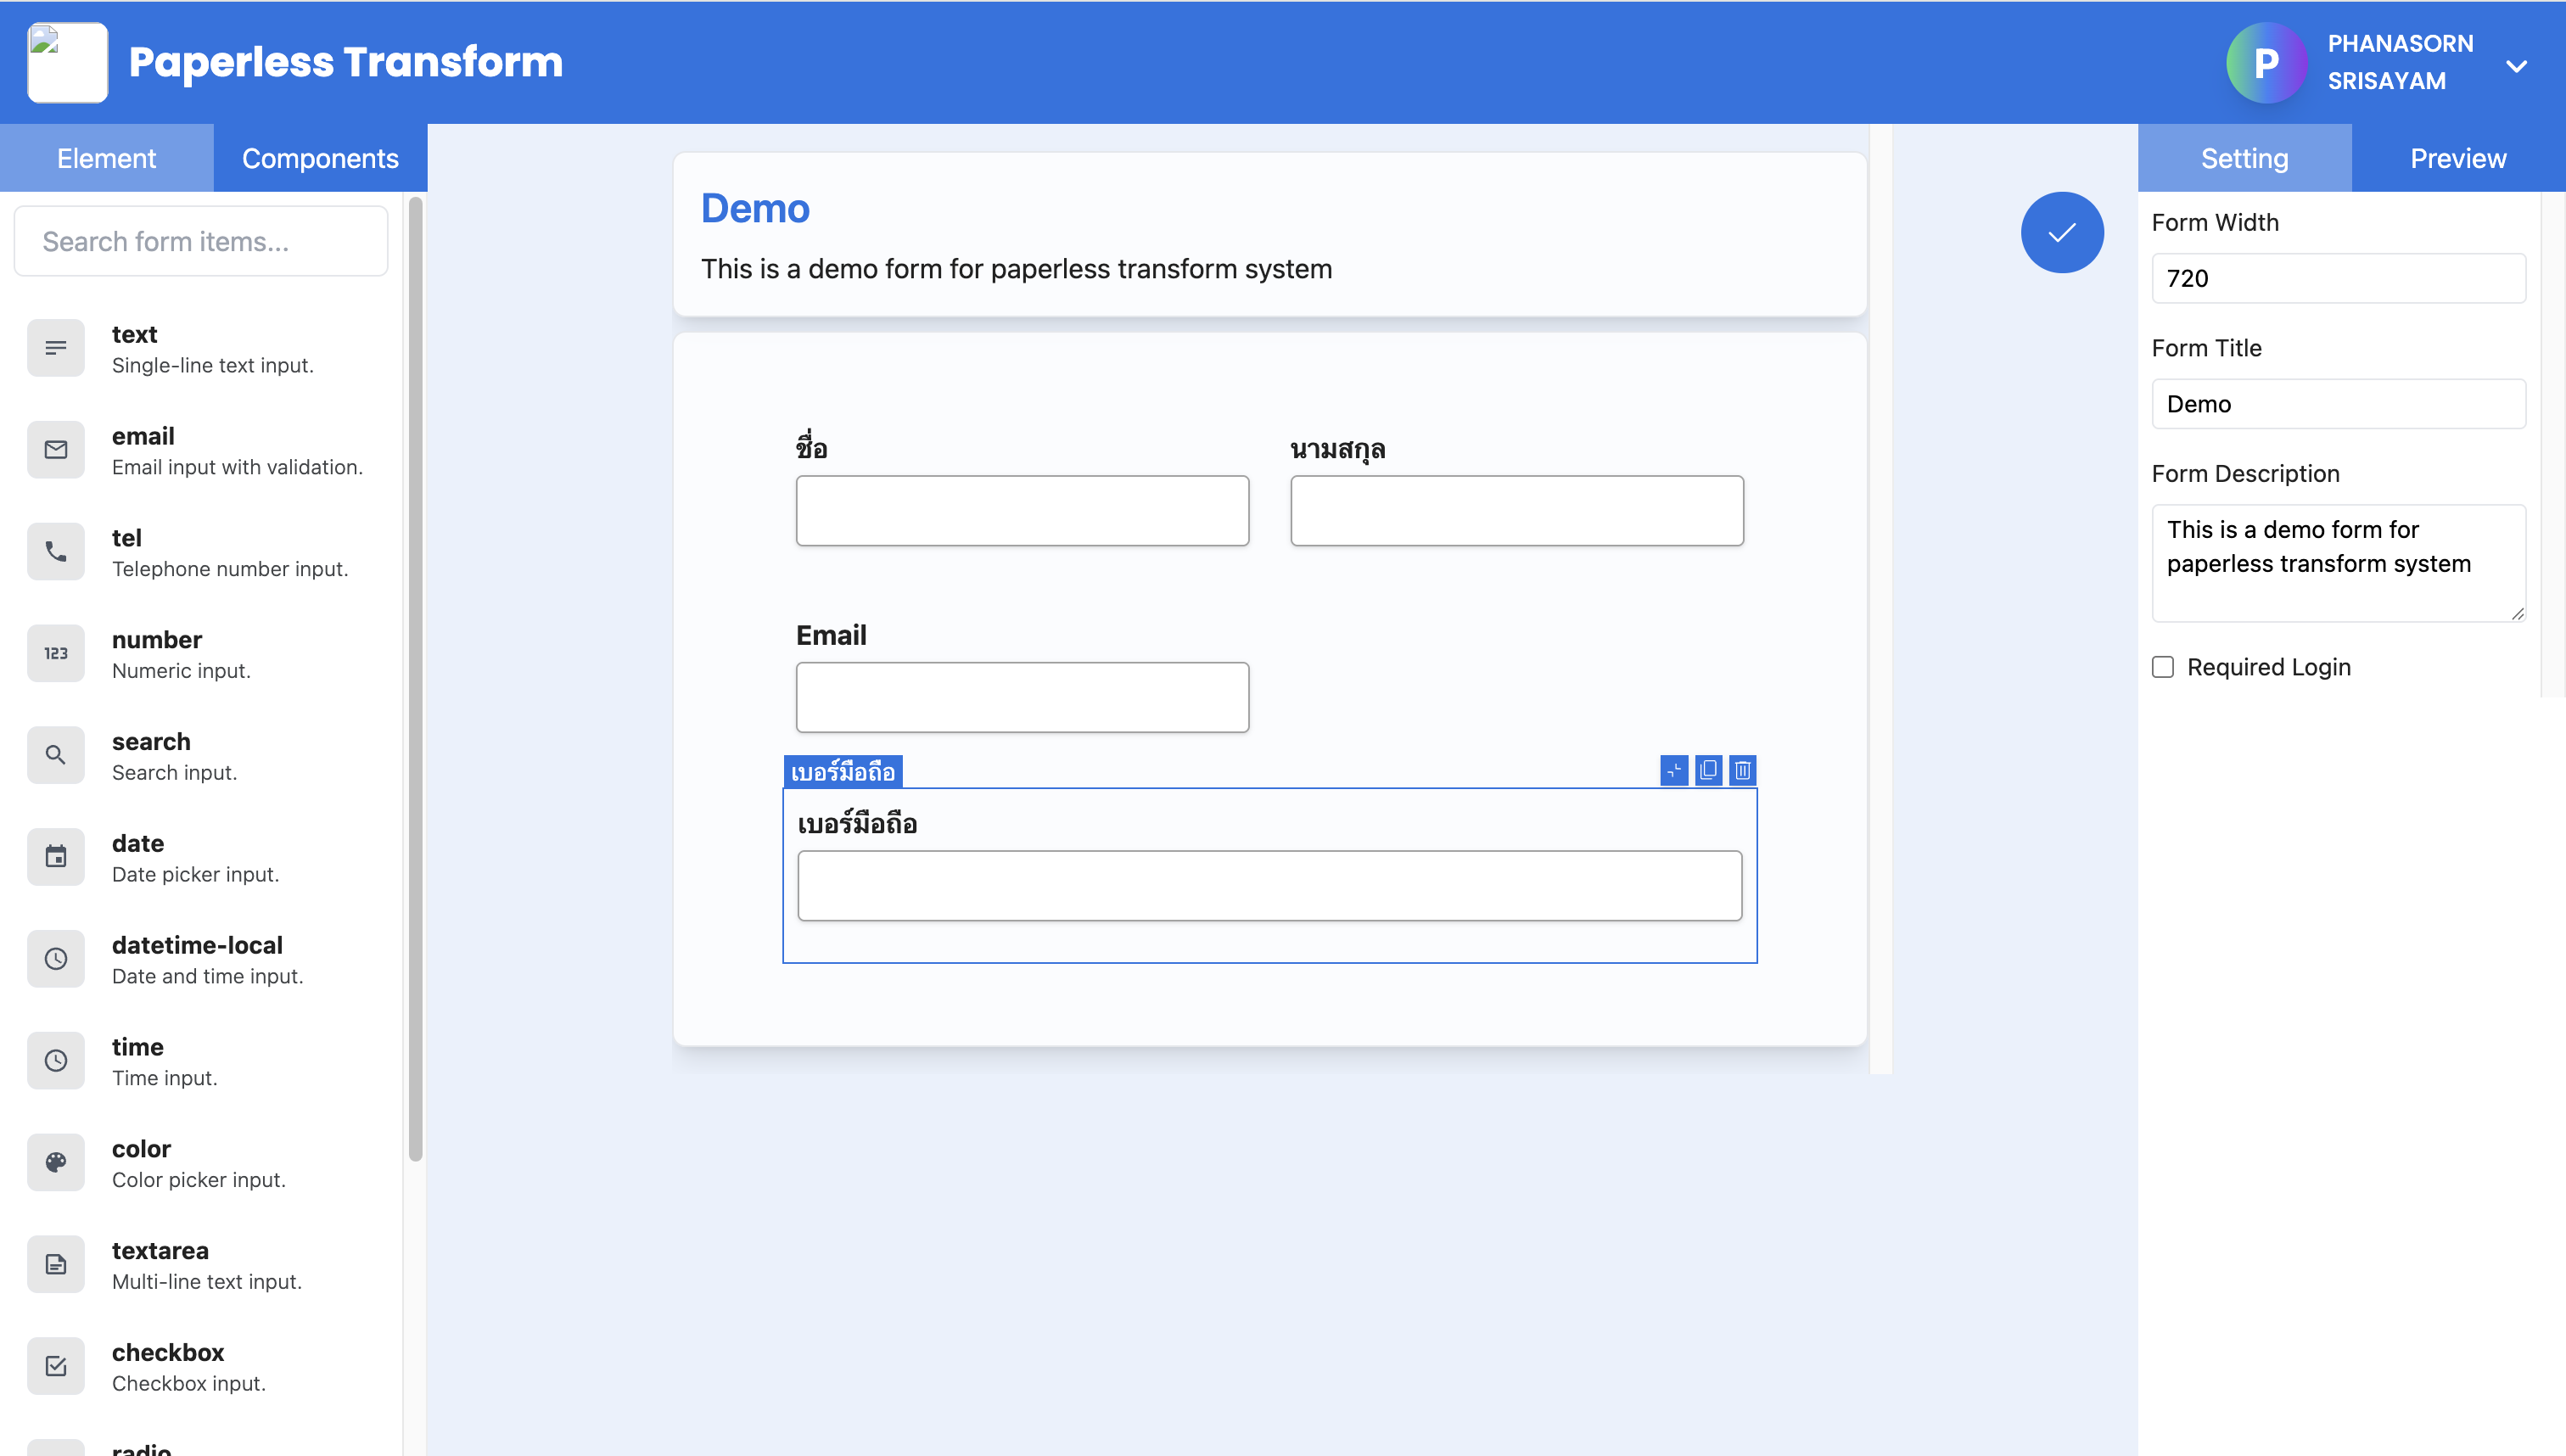
\includegraphics[width= 10cm]{./assets/UI/edit-form.png}}
\caption{Edit Form Page}\label{fig:edit-form}
\end{figure}

Figure \ref{fig:edit-form} represents the Edit Form. The edit form page uses the SurveyJS library, which allows users to fully customize a form, including changing the color, adding a second page, and creating form conditions.

\newpage
\subsection{Form Page}

\begin{figure}[!h]
\centering
\fbox{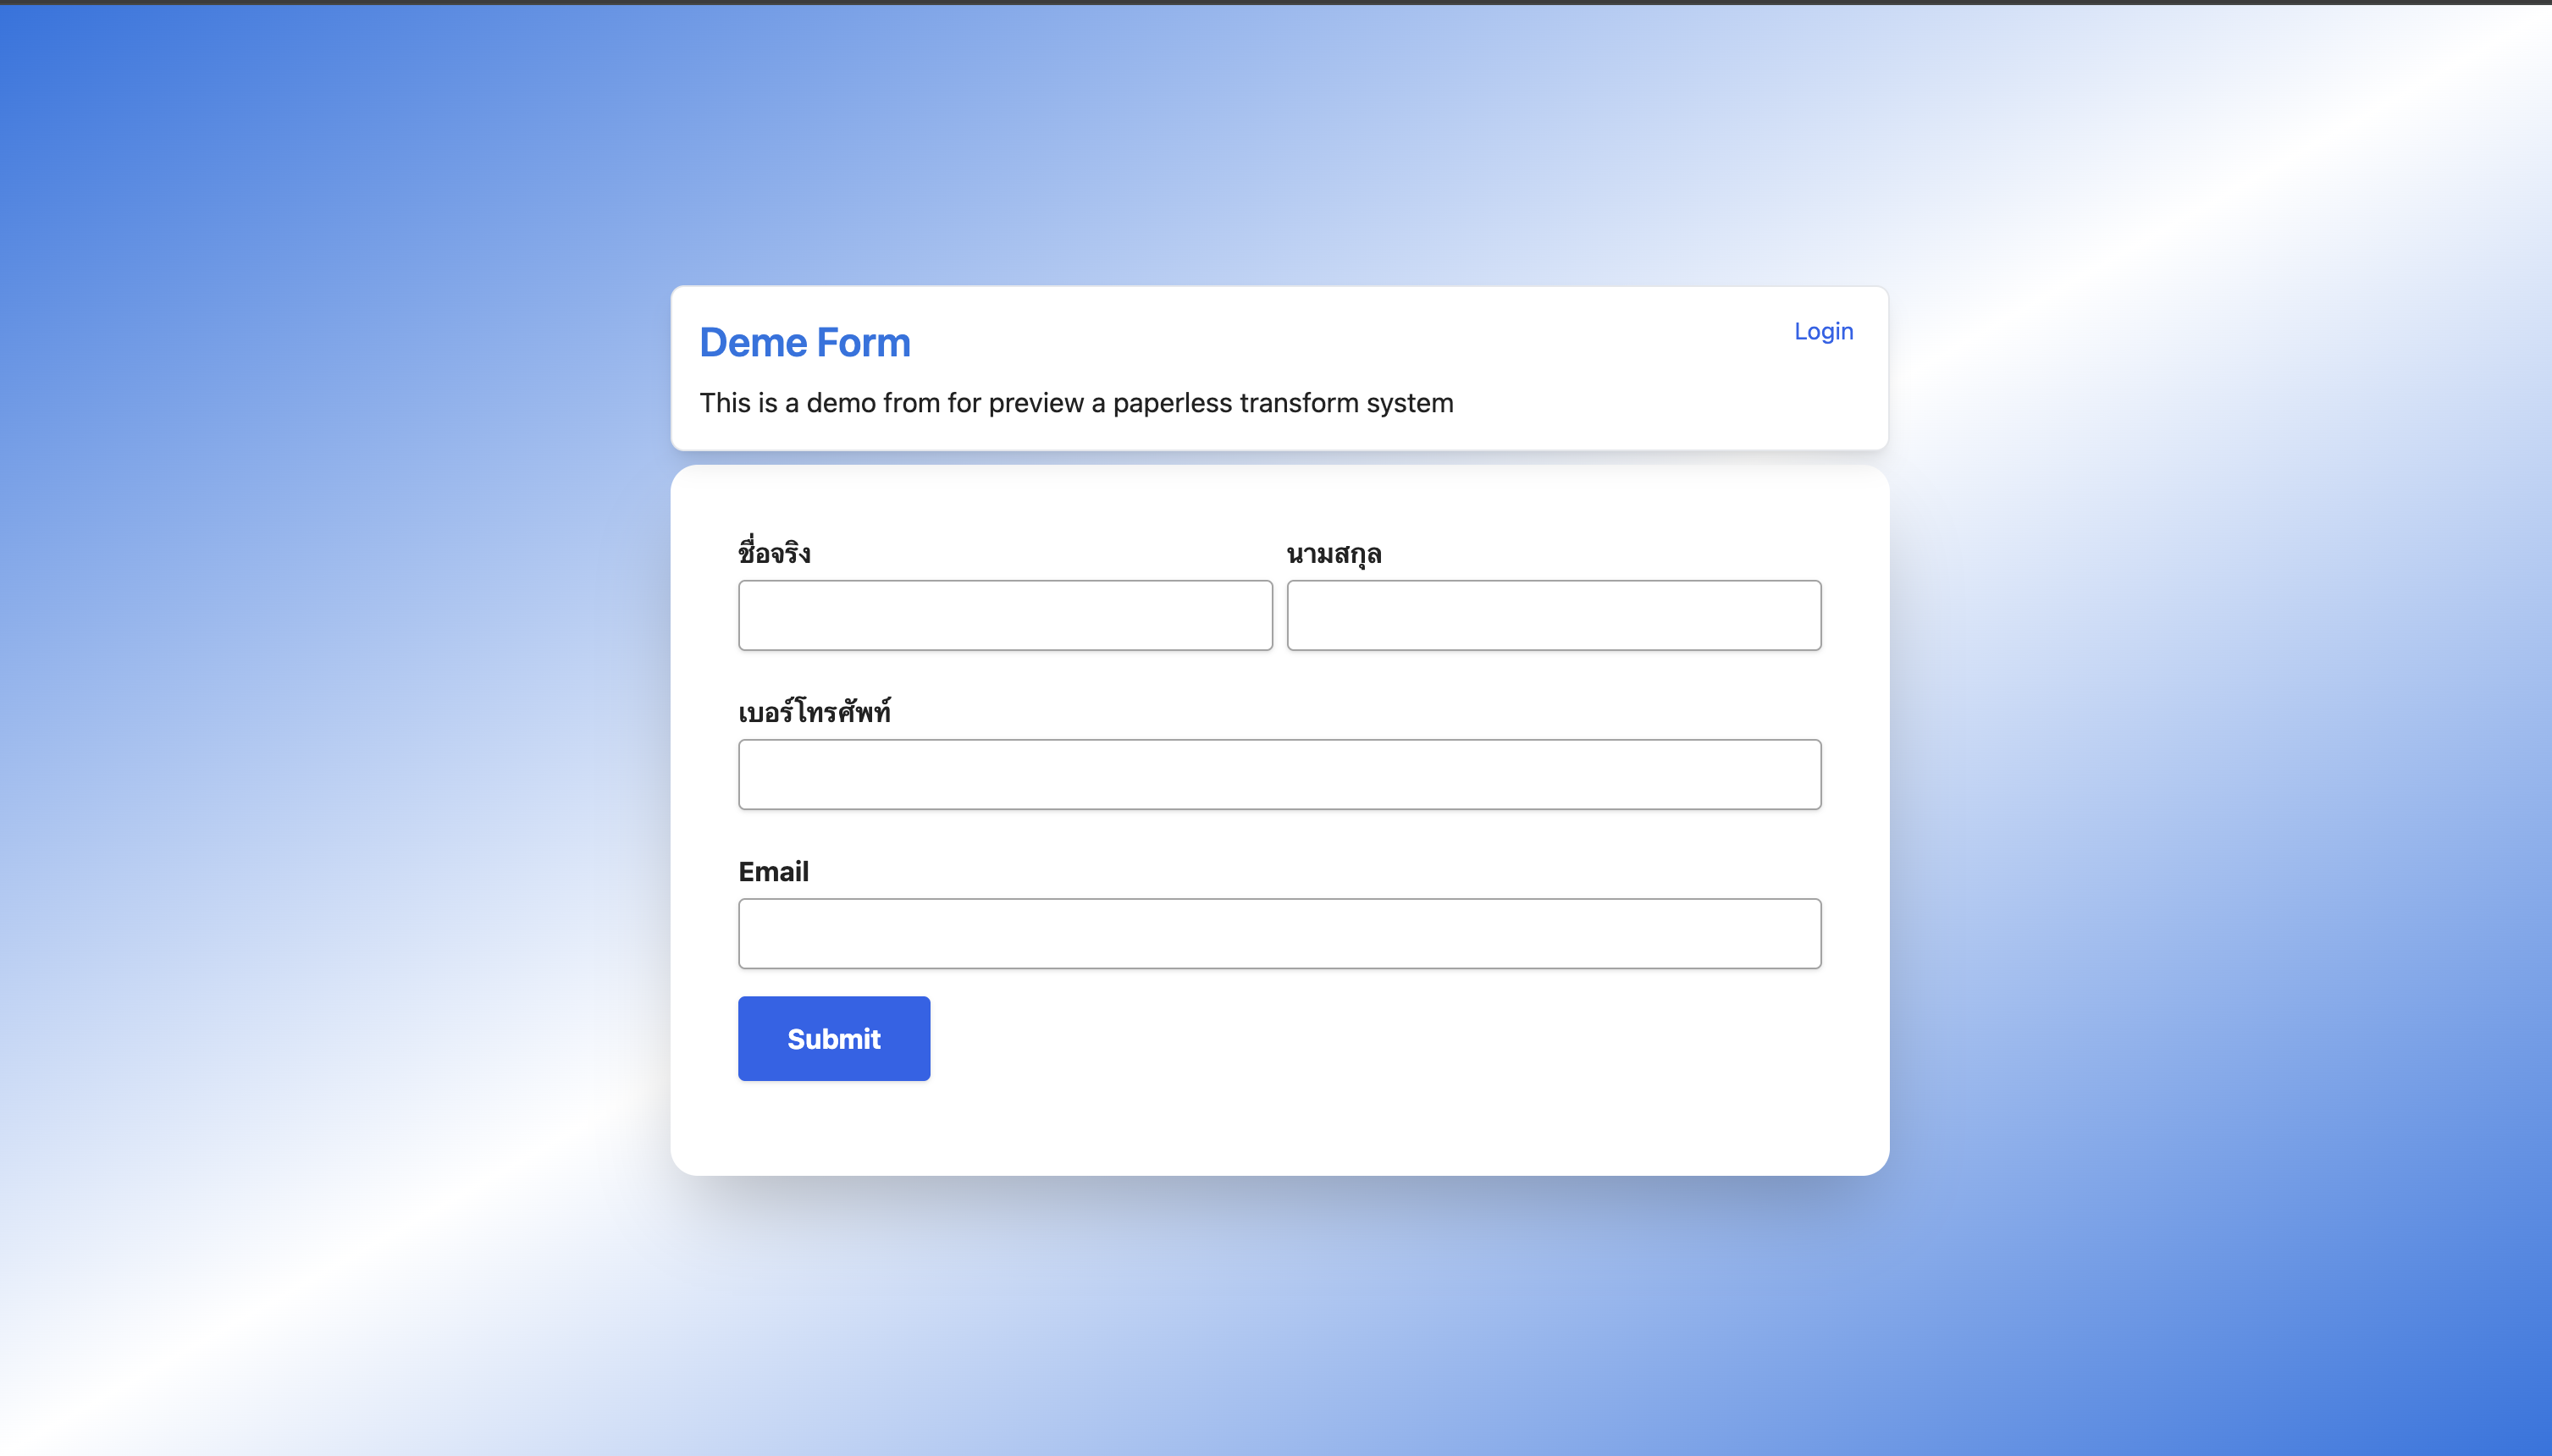
\includegraphics[width= 10cm]{./assets/UI/form-page.png}}
\caption{Form Page}\label{fig:form-page}
\end{figure}

Figure \ref{fig:form-page} showcases the example of web form user interface, which it use a surveyJS to render the UI. This  page will allow user to fill the information and submit a data to the system.


%%%%%%%%%%%%%%%%%%%%%%%%%%%%%%%%%%%%%%%%%%%%%%%%%%%%%%%%%%%%%%
%%%%%%%%%%%%%%%%%%%% Experiments %%%%%%%%%%%%%%%%%%%%%%%%%%%%%
%%%%%%%%%%%%%%%%%%%%%%%%%%%%%%%%%%%%%%%%%%%%%%%%%%%%%%%%%%%%%%%
\chapter{Implementation Results}

You can title this chapter as \textbf{Preliminary Results} or \textbf{Work Progress} for the progress reports. Present implementation or experimental results here and discuss them.


ALL SECTIONS IN THIS CHAPTER ARE OPTIONAL. PLEASE CONSULT YOU ADVISOR AND DESIGN YOUR OWN SECTION

\emph{\textthai{หัวข้อต่าง ๆ ในแต่ละบทเป็นเพียงตัวอย่างเท่านั้น หัวข้อที่จะใส่ในแต่ละบทขึ้นอยู่กับโปรเจคของนักศึกษาและอาจารย์ที่ปรึกษา}}

%%%%%%%%%%%%%%%%%%%%%%%%%%%%%%%%%%%%%%%%%%%%%%%%%%%%%%%%%%%%%%%
%%%%%%%%%%%%%%%%%%%% Conclusions %%%%%%%%%%%%%%%%%%%%%%%%%%%%%
%%%%%%%%%%%%%%%%%%%%%%%%%%%%%%%%%%%%%%%%%%%%%%%%%%%%%%%%%%%%%%%
\chapter{Conclusions}

 \begin{figure}[!h]
\caption{This is how you mention when figure come from internet  \href{https://www.google.com} {https://www.google.com}}\label{fig:x1}
\end{figure}

This chapter is optional for proposal and progress reports but 
is required for the final report.

THIS IS AN EXAMPLE. ALL SECTIONS BELOW ARE OPTIONAL. PLEASE CONSULT YOU ADVISOR AND DESIGN YOUR OWN SECTION

\emph{\textthai{หัวข้อต่าง ๆ ในแต่ละบทเป็นเพียงตัวอย่างเท่านั้น หัวข้อที่จะใส่ในแต่ละบทขึ้นอยู่กับโปรเจคของนักศึกษาและอาจารย์ที่ปรึกษา}}

\section{Problems and Solutions}
State your problems and how you fixed them.

\section{Future Works}
What could be done in the future to make your projects better.

%%%%%%%%%%%%%%%%%%%%%%%%%%%%%%%%%%%%%%%%%%%%%%%%%%%%%%%%%%%%%%%
%%%%%%%%%%%%%%%%%%%% Bibliography %%%%%%%%%%%%%%%%%%%%%%%%%%%%%
%%%%%%%%%%%%%%%%%%%%%%%%%%%%%%%%%%%%%%%%%%%%%%%%%%%%%%%%%%%%%%%

%%%% Comment this in your report to show only references you have
%%%% cited. Otherwise, all the references below will be shown.
%\nocite{*}
%% Use the kmutt.bst for bibtex bibliography style 
%% You must have cpe.bib and string.bib in your current directory.
%% You may go to file .bbl to manually edit the bib items.

% Sept, 2021 by Thanin
% improve url breaks to prevent unnecessary big white spaces in some cases
\makeatletter
\g@addto@macro{\UrlBreaks}{\UrlOrds}
\makeatother
% 

\bibliographystyle{kmutt}
\bibliography{string,cpe}

%%%%%%%%%%%%%%%%%%%%%%%%%%%%%%%%%%%%%%%%%%%%%%%%%%%%%%%%%%%%%%%
%%%%%%%%%%%%%%%%%%%%%%%% Appendix %%%%%%%%%%%%%%%%%%%%%%%%%%%%%
%%%%%%%%%%%%%%%%%%%%%%%%%%%%%%%%%%%%%%%%%%%%%%%%%%%%%%%%%%%%%%%
\appendix{First appendix title}
\noindent{\large\bf Put appropriate topic here} \\

This is where you put hardware circuit diagrams, detailed experimental data in tables or source codes, etc.. \\ \bigskip

 \begin{figure}[!h]
\caption{This is the figure x11 \href{https://www.google.com} {https://www.google.com}}\label{fig:x1}
\end{figure}

This appendix describes two static allocation methods for fGn (or fBm)
traffic. Here, $\lambda$ and $C$ are respectively the traffic arrival
rate and the service rate per dimensionless time step. Their unit are
converted to a physical time unit by multiplying the step size
$\Delta$. For a fBm self-similar traffic source,
Norros~\cite{norros95} provides its EB as
\begin{equation}\label{eq:norros}
  C = \lambda + (\kappa(H)\sqrt{-2\ln\epsilon})^{1/H}a^{1/(2H)}x^{-(1-H)/H}\lambda^{1/(2H)}
\end{equation}
where $\kappa(H) = H^H(1-H)^{(1-H)}$. Simplicity in the calculation is
the attractive feature of (\ref{eq:norros}).

The MVA technique developed in~\cite{kim01} so far provides the most
accurate estimation of the loss probability compared to previous
bandwidth allocation techniques according to simulation results.
Consider a discrete-time queueing system with constant service rate
$C$ and input process $\lambda_n$ with $\mathbb{E}\{\lambda_n\} =
\lambda$ and $\mathrm{Var}\{\lambda_n\} = \sigma^2$.  Define $X_n \equiv
\sum_{k=1}^n \lambda_k - Cn$.  The loss probability due to the MVA
approach is given by
\begin{equation}\label{eq:loss_mva}
  \varepsilon \approx \alpha e^{-m_x/2}
\end{equation}
where
\begin{equation}\label{eq:mx}
m_x = \min_{n \geq 0} \frac{((C-\lambda)n + B)^2}{\mathrm{Var}\{X_n\}} =
\frac{((C-\lambda)n^\ast + B)^2}{\mathrm{Var}\{X_{n^{\ast}}\}}
\end{equation} 
and 
\begin{equation}\label{eq:alpha}
  \alpha =
  \frac{1}{\lambda\sqrt{2\pi\sigma^2}}\exp\left(\frac{(C-\lambda)^2}{2\sigma^2}\right)
  \int_C^\infty (r-C)\exp\left(\frac{(r-\lambda)^2}{2\sigma^2}\right)\, dr
\end{equation}
For a given $\varepsilon$, we numerically solve for $C$ that satisfies
(\ref{eq:loss_mva}). Any search algorithm can be used to do the task.
Here, the bisection method is used.  

Next, we show how $\mathrm{Var}\{X_n\}$ can be determined.  Let
$C_{\lambda}(l)$ be the autocovariance function of $\lambda_n$.  The
MVA technique basically approximates the input process $\lambda_n$
with a Gaussian process, which allows $\mathrm{Var}\{X_n\}$ to be
represented by the autocovariance function.  In particular, the
variance of $X_n$ can be expressed in terms of $C_{\lambda}(l)$ as
\begin{equation}
  \mathrm{Var}\{X_n\} = nC_{\lambda}(0) + 2\sum_{l=1}^{n-1} (n-l)C_{\lambda}(l)
\end{equation} 
Therefore, $C_{\lambda}(l)$ must be known in the MVA technique, either
by assuming specific traffic models or by off-line analysis in case of
traces.  In most practical situations, $C_{\lambda}(l)$ will not be
known in advance, and an on-line measurement algorithm developed
in~\cite{eun01} is required to jointly determine both $n^\ast$ and
$m_x$. For fGn traffic, $\mathrm{Var}\{X_n\}$ is equal to $\sigma^2
n^{2H}$, where $\sigma^2 = \mathrm{Var}\{\lambda_n\}$, and we can find
the $n^\ast$ that minimizes (\ref{eq:mx}) directly. Although $\lambda$
can be easily measured, it is not the case for $\sigma^2$ and $H$.
Consequently, the MVA technique suffers from the need of prior
knowledge traffic parameters.


%%%%%%%%%%%%%%%%%%%%%%%%%%%%%%%%%%%%%%%%%%%%%%%%%%%%%%%%%%
%%%%%%%%%%%%%%% The 2nd appendix %%%%%%%%%%%%%%%%%%%%%%%%%%
%%%%%%%%%%%%%%%%%%%%%%%%%%%%%%%%%%%%%%%%%%%%%%%%%%%%%%%%%%
\appendix{Second appendix title}
\noindent{\large\bf Put appropriate topic here} \\


 \begin{figure}[!h]
\caption{This is the figure x11 \href{https://www.google.com} {https://www.google.com}}\label{fig:x1}
\end{figure}

Next, we show how $\mathrm{Var}\{X_n\}$ can be determined.  Let
$C_{\lambda}(l)$ be the autocovariance function of $\lambda_n$.  The
MVA technique basically approximates the input process $\lambda_n$
with a Gaussian process, which allows $\mathrm{Var}\{X_n\}$ to be
represented by the autocovariance function.  In particular, the
variance of $X_n$ can be expressed in terms of $C_{\lambda}(l)$ as
\begin{equation}
  \mathrm{Var}\{X_n\} = nC_{\lambda}(0) + 2\sum_{l=1}^{n-1} (n-l)C_{\lambda}(l)
\end{equation} 

\noindent{\large\bf Add more topic as you need} \\

Therefore, $C_{\lambda}(l)$ must be known in the MVA technique, either
by assuming specific traffic models or by off-line analysis in case of
traces.  In most practical situations, $C_{\lambda}(l)$ will not be
known in advance, and an on-line measurement algorithm developed
in~\cite{eun01} is required to jointly determine both $n^\ast$ and
$m_x$. For fGn traffic, $\mathrm{Var}\{X_n\}$ is equal to $\sigma^2
n^{2H}$, where $\sigma^2 = \mathrm{Var}\{\lambda_n\}$, and we can find
the $n^\ast$ that minimizes (\ref{eq:mx}) directly. Although $\lambda$
can be easily measured, it is not the case for $\sigma^2$ and $H$.
Consequently, the MVA technique suffers from the need of prior
knowledge traffic parameters. 





\end{document}
